\chapter{Introduction}

Artificial Chemistries of discrete atoms provide an interesting testbed
for investigating various evolutionary phenomena. Fundamentally, they
provide a tuneable evolutionary system, capable of highly complex
behaviour, built around familiar metaphors (real-world Chemistry, and
potentially Biology). A set of interaction rules describing how atoms
interact gives rise to emergent forms -- molecules. At a higher level,
these molecules, under the same interaction rules, also interact in
patterns -- reactions.

\TODO{ link emergent levels to copy mechanism}

Still higher emergent levels emerge under favourable conditions.
Reactions may form cycles, where a sequence eventually returns to an
earlier product. Our interest is in identifying the factors that
influence the emergence of these higher levels. Cycles in particular are
interesting as many biological processes are cyclical. Replication,
resulting in an exact copy of an entity, is a macro-example of a cycle;
metabolism is another. Building on the apparent correspondence between
higher emergent levels in Artificial Chemistry evolution and Biology, we
believe like others (e.g., \autocite{Steel2013}) that cycles, of some
form, are a necessary building-block for more complicated structures
again in Artificial Chemistries.

\TODO{ argue that ToyWorld capable of a tunable copying mechanism, similar to that in biology,
	but that such a mechanism will be difficult to evolve de novo. Previous work on
	evolution of a DNA/RNA copy mechanism in biology: Eigen's paradox, fidelity requires error-correction,
proteins etc}

\section{Contributions}

\begin{enumerate}
	\item
 Open-sourced Artificial Chemistry model
	\item
 Progress towards useful heredity in an artificial system
	\item
 Progress towards OEE in artificial system--evolution compatible with
 OEE without necessarily showing OEE (which is hard to measure and
 prove)
	\item
 Demonstration of formation of ACS in an artificial chemistry (previous
 work with ODEs e.g. \autocite{Hurndall2014} not re-usable in that form)
\end{enumerate}

\subsection{Hypothesis}\label{hypothesis}

Because an Artificial Chemistry
\begin{itemize}
	\item
 Meets known constraints for OEE--and we have OOL as an example of OEE
 from natural chemistry
	\item
 Choosing an artificial chemistry similar to natural chemistry enables
 an argument by analogy
	\item
 Catalysis/autocatalysis possible through emergence in some AChems
 (e.g., \autocite{Virgo2013})
	\item
 And TODO..
\end{itemize}

Hx: Compliant copy-mechanism possible in an AChem through analogy with DNA/RNA copying

\chapter{Artificial Chemistries}\label{artificial-chemistries}

\section{Introduction}\label{introduction-2}

Full taxonomy in \autocite{Dittrich:2001zr}, also see \autocite{Faulconbridge2011}

One advantage of \glspl{achem} as pointed out by
\autocite[5]{Funes2001} is that it is easier to evaluate solutions in
a domain close to the real-world as opposed to a purely symbolic or
abstract domain such as a lambda-calculus, or a programmatic environment
like Tierra. When contemplating difficult problems such as complexity
our intuition can be helpful, but only in situations close enough to our
normal experience for it to be relevant.

All Artificial Chemistry based on this model:

\begin{figure}[t]
	\begin{center}
		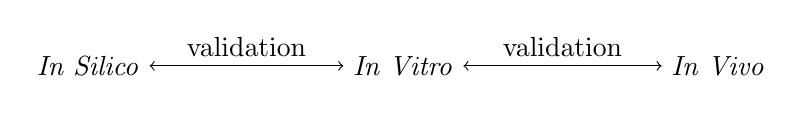
\begin{tikzpicture}
			\node (silico) at (0,0) {\textit{In Silico}};
			\node (vitro) at (4,0) {\textit{In Vitro}};
			\node (vivo) at (8,0) {\textit{In Vivo}};
			\draw [<->] (silico) -- (vitro) node [midway,above] {validation};
			\draw [<->] (vitro) -- (vivo) node [midway,above] {validation};
		\end{tikzpicture}
	\end{center}
\end{figure}

Or in other words, digital models (``in silicon''), wet-chemistry models
(``in glass''), and life itself.

In general, AChems for these problems are without grounding (so start
from high-level). Grounding implies that there is a causal justification
for the higher level chemistry, where that justification is based on
fundamental supportable processes, rather than unique to particular
problem.

All four areas rely on a connection to real chemistries--Molecular
synthesis and Molecular Programming require results to be transferrable
to In Vitro; other two expect results to shed light on In Vivo
processes.

Therefore expect that a grounded AChem for these should have a basis in
real Chemistry.

\subsection{BOX--Physical or Real-world Chemistry}\label{box -- physical-or-real-world-chemistry}

The richness of the real world is built on a substantial foundation of
chemical and physical complexity.

A \textit{reaction} transforms \emph{reactants} into \emph{products},
and is often represented by describing the quantities (or stoichiometry)
of reactant and resulting product molecules. The reaction can also be
characterized by a description of the dynamics, or kinetics, of the
reaction to explain how the reaction proceeds in response to temperature
changes or to varying concentrations of reactants. Reactions often
require an input of energy, such as from molecular collisions, to
proceed; the energy required is called the reaction's activation energy
(\(A_e\)), and is specific to the particular reaction. In general there
is no accurate mechanism to predict reaction dynamics without
experiment.

The \textit{reaction rate} is the change in concentration of a substance
over time: \(\frac{-d[A]}{dt} = k[A][B]\) (where the notation \([X]\)
means that concentration of \(X\) and \(k\) is the reaction rate
constant) leading to Arrenhius' description of the relationship between
the activation energy (\(E_a\)), the temperature (\(T\)) and the rate
constant (\(k\)): \(k = Ae^{E_a/RT}\). The \textit{reaction order}
describes how the reaction rate changes with the concentration of the
reactants, usually captured as a first-, second-, or third-degree
polynomial expression determined empirically. For example, the reaction
rate equation for \(2NO + Cl_2 \rightarrow 2NOCl\) is
\(rate = k[NO]^2[Cl_2]\) (experimentally determined), and is
second-order with respect to \(NO\), first-order with \(Cl_2\) and
overall (the sum of terms), third-order. (Example taken from
\autocite{Kotz2006})

Reactions in theory can be decomposed to a chain of
\emph{elementary steps}, with each step resulting in a single change,
such as bond formation or cleavage, to the reacting molecules.
Elementary steps are somewhat predictable, practical reactions somewhat
less so. Generally in experimental chemistry we know the reactants and
products and can sometimes deduce the sequence of elementary steps.

In modelling, we can either represent reactions exactly as an atomic
transformation from reactants to products with characteristics that can
only be determined experimentally, or we can attempt to construct the
reaction from a sequence of elementary steps with the properties of the
reaction derived from the properties of the steps involved. This later
approach is the only practical one when the reaction is novel, or when
we lack experimental data. Several alternate sequences of steps, or
\textit{reaction pathways}, may be possible between reactants and
products. Each pathway will have a different activation energy, and
hence reaction rate.

The kinetics of elementary steps are defined by the stoichiometry of the
step and are hence predictable. In theory you might expect to be able to
predict the overall reactions kinetics from the composition of these
elementary steps. In practice, the results are close, but not exact,
when compared to experiment. However they form a useful abstraction for
analysis. The reaction rate of an elementary step is defined by the
stoichiometry, where the rate equation is the product of the reactant
concentrations and the rate constant. Therefore a step with one reactant
has order 1, a bimolecular step (\(A + B\)) has order 2 and so on. The
step \(2A + B\) has rate equation \(k[A][A][B] = k[A]^2[B]\) and is of
order 3.

Elementary steps are an abstraction, an aid to analysis, of the
underlying molecular dynamics. At the molecular level, reactions can be
modelled as a series of collisions between molecules. The reaction rate
is then determined by the percentage of collisions (or in other words,
the concentration) that are energetic enough to overcome the inherent
stability of the interacting molecules and cause a change in molecular
structure or shape (in other words, the activation energy).

Recall that the rate of a reaction is a function of concentration (at
the gross level) or collision rate (at the molecular level) and the
activation energy for the reaction, which at the molecular level is
directly related to the energy required to overcome the stability of the
reactants. There are therefore two clear mechanisms to alter the rate
for a reaction: either reduce activation energy, or increase
concentrations. A catalyst does precisely the first, and autocatalysis
is one method for the second.

A catalyst is anything that isn't consumed by the reaction and that
affects the rate (or the kinetic equation for the reaction) without
affecting the reaction's equilibrium constant. Catalysts allow the
reaction to proceed by an alternate, lower activation energy, pathway.
The reaction equation remains the same, but the dynamics are changed -
in the case of biological enzymes the rate can be increased by several
orders of magnitude over the uncatalyzed reaction, enabling reactions
fundamental to life that would be effectively impossible in an
uncatalysed form. At the molecular level catalysts often function by
providing a substrate that preferentially attacks the bonds critical to
the reaction. The platinum within an automotive catalytic converter is a
well-known example of a catalytic substrate.

Autocatalysis, introduced by \autocite{Ostwald1890}, is a different
approach to catalysis. Rather than reducing the required activation
energy, autocatalysis increases the reactant concentrations:
autocatalysis reactions form feedback loops where a compound is both a
reactant and a product. In the standard definition, an autocatalytic
reaction is one that is catalysed by its own products, resulting in a
characteristic rate acceleration over time given by the differential
equation -
\[\frac{dx_i}{dt} = k(\mathbf{X}) \cdot x^n_i + f(\mathbf{X})\] where
\(n\) is the order of the reaction \autocite{Plasson2010}. Example
(indirect network autocatalysis) of glycolysis where pattern is ATP
\(\rightarrow\) n.ATP--ATP initially consumed, but overall created.

Autocatalysis may be realised by 1) either a single reaction (\eg A + X
+ Y \(\rightarrow\) 2A + Z) or a linear chain of reactions through
intermediate products, called template autocatalysis, or 2) by a
reaction network. Networks may be indirect through a series of
intermediary products, or collective where there is no connection
between the component cycles other than through catalysis--as seen for
example in the replication of viroids where each RNA strand can catalyse
the production of the other. However, in all cases, the reactions reduce
to the defining X \(\rightarrow\) nX pattern described by Ostwald's
differential equation.\autocite{Plasson2010}.

A related phenomenon is autoinduction where products increase the
reactivity of the catalyst (rather than directly affecting the reaction
mechanism). Same signature (Ostwald).

Artificial chemistries are regularly employed in three application
areas: real-world chemistry emulators; tools for the exploration of
artificial life, and models to test various hypotheses of the origin of
life. Chemistry emulators and origins-of-life tools aim for fidelity
with real-world chemistry, unlike most artificial life models.
Real-world fidelity requires either the use of a library of predefined
reactions, which conflicts with the goal of unlimited extension, or a
chemically plausible method of constructing reactions from first
principles. Because of the complexities of real-world chemistry this
later method appears to be quite difficult, and the goal of a realistic,
computationally practical, artificial chemistry remains open. However,
the more limited objective of a less realistic, but still fully
constructive chemistry, has been achieved (see Table \cref{classification-of-artificial-chemistries} for
examples.). A constructive chemistry (\autocite{Fontana1994}) is one
where new components may be generated through the action of other
components, and where those new components may themselves take part in
new types of reactions, and so on. This appears fundamental to an
open-ended representation.

A mathematical treatment of \gls{achem} can be found in
\autocite{Benko2009}. \autocite{Dittrich:2001zr} and
\autocite{Suzuki2008a} provide excellent reviews of the field.

\section{Classification of Artificial Chemistries}\label{classification-of-artificial-chemistries}

In \autocite{Dittrich:2001zr}, Achems divided into major types:

\begin{itemize}
	\item
 Rewriting or Production Systems (symbols and rewriting rules) -
 Chemical Abstract Machine (CHAM), Chemical Rewriting System on
 Multisets (ARMS), Chemical Casting Model (CCM), Lambda-Calculus
 (AlChemy)
	\item
 Arithmetic Operations (molecules are natural numbers, operations are
 arithmetic operators)
	\item
 Autocatalytic Polymer Chemistries (polymers made from chains of
 monomer symbols, reactions are concatenation and cleavage)
	\item
 Abstract Automata and Artificial Molecular Machines (seem similar)
 e.g., Turing
	\item
 Assembler Automata--Avida, Tierra
	\item
 Lattice Molecular Systems--\autocite{Ono2000},Madina2003,lattice
 molecular automaton (LMA), Autopoietic System
\end{itemize}

A \gls{achem} can be represented by
\textless{}\emph{S},\emph{R},\emph{A}\textgreater{}
\autocite{Dittrich:2001zr}:

\begin{itemize}
	\item
 Set of Molecules (\textless{}\emph{S}\textgreater{})
\end{itemize}

Molecule representation e.g., labelled graphs

Properties of molecules e.g., energy calculation by Extended Huckel
Theory (EHT); salvation energies; reaction rates.

\begin{itemize}
	\item
 Reaction rules (\textless{}\emph{R}\textgreater{}) (Chemistry)
\end{itemize}

Transformation from lhs reactants to rhs products. Many (most) reactions
are bidirectional; rates determined by concentrations. Conservation of
energy ? atoms are neither created or destroyed so reactions can be
represented solely by bond changes.

Chemical Abstract Service (CAS) database references approx 34 million
reactions in published work (1) Which ones to adopt? Which reactions
direct evolution to more interesting places?

Reactions may be pre-defined (if S represents real-world molecules) or
dynamically-determined using molecular properties--the problem of how
to select a reaction is addressed by the Reactor Algorithm (below.)

\autocite{Tominaga2007} showed for a particular artificial chemistry,
that it is computationally universal with only unimolecular and
bimolecular reactions.

\begin{itemize}
	\item
 Reactor Algorithm (\textless{}\emph{A}\textgreater{}) (Physics)
\end{itemize}

Mechanism to select reactions, e.g., Through the introduction of a
reaction generator (A) the artificial chemistry triplet (S, R, A) is
completely defined \autocite{Lenaerts2009}. Or in
\autocite[sect. 4.1.3]{Faulconbridge2011}, The mixing component of an
Artificial Chemistry is an algorithm which describes the order of and
intervals between reactions, starting from an initial collection of
molecules; this can be termed a ``mixing space''.

\autocite{Faulconbridge2011} identifies three types of
\emph{mixing method} or reactor algorithm:

\begin{itemize}
	\item
 Well-mixed/aspatial: with either discrete time (uniform probability
 distribution for selecting reactions) or continuous time
 (Gillespie1976) assuming the reactions are known in advance (not
 possible for a strongly constructive AChem)
	\item
 nDimensional: grid with reactions with adjacent cells, or continuous
 where molecules have position and velocity. Major advantage is ability
 to simulate spatial affects; disadvantage is performance
	\item
 Mixed scale: hierarchical spaces, such as aspatial cells within bigger
 grid, mostly for simulating biology (e.g., \autocite{Jeschke2008}). One possible
 advantage is potential for parallelization
\end{itemize}

Scaling can be an issue: as new products are generated, the space of
reactions and reactants can expand exponentially, and therefore
performance dives. The general problem is model reduction--see
\autocite{Radulescu2012} for a recent review; \autocite{Faulon2001} has
a well-received method.

Alternative classification in \autocite{Faulconbridge2011}:

\begin{itemize}
	\item
 Symbolic--each molecular species labelled by a unique symbol; only
 explicit meanings
	\item
 Structured Symbolic \eg \autocite{Hutton2002}--standard, hard to achieve
 emergence or support novel molecules
	\item
 Sub-symbolic \eg RBN-World, NAC, ToyChem \autocite{Benko2005}
\end{itemize}

\subsection{Constructive chemistries}\label{constructive-chemistries}

Novel molecules can arise from artificial chemistry:

\quote{
	A distinguishing feature of chemistry is that the changes of molecules
	upon interaction are not limited to quantitative physical properties
	such as free energy, density, or concentrations, since molecular
	interactions do not only produce more of what is already there --
rather, novel molecules can be generated.}
{\autocite{Benko2009}}

A chemistry is \textit{constructive} \autocite{Fontana1994} if new components
may be generated through the action of other components. Both implicit
laws and implicit molecule definitions are required for constructive
chemistries:

\begin{itemize}
	\item
 Explicit reaction laws = independent of molecular structure; implicit
 = laws must refer to structure. Often used for constructive
 chemistries
	\item
 Explicit molecule definitions = from an fixed set of symbols; implicit
 = description for construction.
\end{itemize}

Constructive (weak and strong) initially defined in \autocite{Fontana1994}:

\quote{
	We refer to models in which new agents are constructed in an unspecific
	(essentially stochastic) fashion as \emph{weakly constructive}. This is
	to be contrasted with a situation in which the encounter of two agents
	\emph{implies} a \emph{specific} third one\ldots{}Models of this kind
	will be termed \emph{strongly constructive}. The prime example of a
strongly constructive system is chemistry.}
{\autocite{Fontana1994}}

The commentary that immediately follows is also significant:

\quote{
	A strongly constructive system that contains agent \emph{A} must cope
	with the network of its implications. But, then, it also must cope with
the implications of the implications. And so on.}
{\autocite[217]{Fontana1994}}

A strongly constructive system is one which maintains closure, and in
which there is self-consistency and some form of logical structure
(implications.)

A mechanism for exploration in the EA sense--new products can be
generated, and new products can participate in reactions. One approach
is to pre-specify all possible reactions; another is to generate
reactions `on-the-fly' from the structures of the interacting molecules.
The first approach is well suited to simulating real chemistry as it
allows properties of reactions observed in chemical experiments to be
attached to their simulated equivalents. However, it does not allow for
arbitrary reactions, and it requires reaction properties to be
pre-specified--difficult for novel or artificial reactions. It could be
argued that the first approach is not in fact strongly constructive (in
the sense of \autocite{Fontana1994,Dittrich:2001zr}) as it is not completely
open-ended. However, \autocite{Hartenfeller2011} suggests that it is in fact
adequate.

\subsection{Applications in real-world chemistry}\label{applications-in-real-world-chemistry}

Modeling chemical reactions (\eg \autocite{Gibson:2000kx}). Emulators
are often used for backward chaining from a set of desired products to
identify a set of currently-available initial molecules, for example in
drug discovery (e.g., \autocite{Hartenfeller2011}). A second use is in
reaction network discovery, where the goal is to describe a closed set
of reactions and reactants from some initial reactants and reactions
(e.g., \autocite{Faulon2001}). Both applications effectively produce
static descriptions of dynamic processes, and are less useful for
exploring the changes in a network over time.

\autocite{Hartenfeller2012} suggests that
R=\{set of 58 reactions\} might meet requirements for de-novo drug
discovery, but based on S=\{10k-50k building-block molecules\}. Given
much smaller S, will this R still suffice?. Goal of identifying
collection of synthesis reactions that can be used by tools to construct
pathway from provided building blocks to desired compounds. Set of 58
reactions, 29 of which are ring-forming, implemented in reaction-SMARTS
and RDKit.Previous work deficient in its potential to generated
innovative chemo-types, because of the small number of ring-forming
reactions (only 3 ring-formations versus 29 in this work.) Why is a
small set of reactions (50-60) adequate? Most reliable, so transferrable
to bench-top; with reasonable collection of building-blocks (10k-50k)
can fill combinatorial space beyond ability to enumerate. Even with this
set need search mechanism to limit combinatorics.

The primary requirement is fidelity with real-world chemistry, which
requires either a library of empirically derived reaction definitions
and rates, or a model capable of accurately simulating
quantum-mechanical processes. The latter approach has been taken by a
family of Artificial Chemistries, beginning with
\autocite{Benko2003}, built on Extended H\"{u}ckel Theory with parameters
taken directly from chemical experiments and later extended (for example
in \autocite{Benko2005}) to a general purpose model with parameters
derived from theoretical chemistry. The model was used in
\autocite{Hogerl2010} for the study of the behaviour and topology of
chemical reaction networks, specifically Diels-Alder and Formose
reaction networks, and in a series of papers (e.g, \autocite{Flamm2010}
and \autocite{Ullrich2010}) for the examination of the evolution of
metabolic networks in early organisms using a simple model of RNA coding
for catalysts.

An artificial chemistry with the ability to create reactions
``on-the-fly'' given a set of possible reactants may discover more than
one possible reaction pathway between the same reactants and products.
The method used to choose one reaction pathway from the alternatives is
an important component of the artificial chemistry, and the mechanism
may be tuned or tailored to privilege or preferentially chose particular
types of pathways independent to other factors such as temperature or
concentration. In Chemistry the choice of reaction pathway is
fundamentally linked to those other properties and cannot be treated
independently.

Rather than from symbol manipulation, Chemical properties emerge from
fundamental laws. This gives a richness and depth that cannot easily be
equalled in a simulation. For example, the three-dimensional structure
of a molecule--the arrangement of the elements in space--drives even
the simplest chemical reactions. Any (base- or acid) reaction results
from the shift of charge from one region of a molecule to another,
revealing one region while shielding another from activity. Some of the
most complex reactions are shape-driven: the function of many enzymes
(biological catalysts) derives from their shape, and furthermore this
shape is often under regulatory control. A cell can in affect regulate
the activity of an enzyme by either blocking or unblocking the enzymes
active site with another protein. The prediction of the shape and hence
the function of an enzyme from its RNA transcript is perhaps the most
important problem in current molecular biology. In \gls{achem}, an
interesting, but highly simplified, attempt at this can be found in the
work of \autocite{Flamm2010} and \autocite{Ullrich2010}.

Investigating natural selection for chemical evolution
(\eg \autocite{Fernando:2007pf})

Reaction network discovery and Drug discovery

\begin{itemize}
	\item
 Chemical Abstract Service (CAS) database references approx 34 million
 reactions in published work
	\item
 Either from products back to reactants, or enumeration of all products
 from reactants
	\item
 describe a closed set of reactions and reactants from some initial
 reactants and reactions (e.g., \autocite{Faulon2001}
	\item
 Realism fundamental
	\item
 There is an inbuilt tension between realism and speed in artificial
 chemistries. Realistic reaction selection must involve calculations of
 likelihood, where the current state of the art is to use quantum
 chemistry simulators to determine the properties of a particular
 reaction. Each reaction that fires alters molecular quantities, and in
 models based on a Gillespie-like method, requires the recalculation of
 the firing probabilities for all affected reactions.
	\item
 The field has generally progressed from simpler, abstract models (such
 as \autocite{Fontana1992}) to more chemically-realistic ones
 \autocite{Suzuki2008a}.
	\item
 Examples
	\item
 \autocite{Hogerl2010} etc--Diels-Alder and Formose reaction networks
\end{itemize}

\subsection{Origins of Life}\label{origins-of-life}

Of the historic and ahistoric aspects of the Origin-of-life problem,
historic aspect may never be known \autocite{Pross2013}. Constrained by
what we do know, but many different pathways, and unless some record
somewhere (either geological or phylogenetic), actual path essentially
lost to history. So without evidence for historic aspect, not possible
to test by falsification, and hence can only be speculative.

Consensus forming that early life formed by chemoautotrophs with energy
from inorganic redox couples and biomass from CO\textsubscript{2}, and
that innovations in carbon-fixation created main branches in
tree-of-life \autocite{Braakman2012}. Initiation of selection marked by
\gls{ida}, probably from RNA world, followed substantially later by Last
Universal Common Ancestor (LUCA) \autocite{Yarus2011}, which, it is
important to note for clarity, was almost certainly not a single cell or
even species, but rather a construct of evolutionary genetics because of
the likely predominance of Lateral Gene Transfer (LGT) in archaic
biology (http://sandwalk.blogspot.ca/2007/03/web-of-life.html).
Self-replicating RNA enzymes shown in \autocite{Lincoln2009}, forming
basis of selective system (link to natural selection) (also see
\autocite{Cheng2010}, \autocite{Powner2009} for formation of RNA in
prebiotic conditions). Some elements of \gls{ida} thought still with us
in lineages of informational (for protein synthesis and RNA
transcription) and operational genes (for some standard cellular
processes) \autocite{Ragan2009}, for example the ribosome and
ribonuclease P (RNase P) \autocite{Wilson2009}. Next major transition to
Protein world (although predominance of RNA transcripts leads to
suggestions that should be called RNA-Protein world
\autocite{Altman2013})

Two alternative models for the step from abiotic to \gls{ida}: genetic
or replicators or RNA-first, and metabolism or protein-first. Both
metabolism and replication almost certainly required for \gls{ida}. A
self-sustaining autocatalytic network (in terms of a RAF set
specifically a ``set of molecules and reactions which is collectively
autocatalytic in the sense that all molecules help in producing each
other (through mutual catalysis, and supported by a food set).'')
generally considered essential \autocite{Pross2013}, but not sufficient
\autocite{Hordijk2011}. Both competing models--replication first and
metabolism first--build on that. Autocatalysis expressed by
self-replication of oligomeric compounds in replication first; by cycles
and network in metabolism first. In the broadest sense, life can be seen
as an autocatalytic process where an entity catalyses the production of
one or more descendant entities.

Metabolism-first privileges function, while replicator-first privileges
descent.

If life is metabolism plus information, then for metabolism-first where
lack template-based replication, replication is compositional (composome
- Vasas)

Common functions required in both protocells and minimal cells, but
approaches quite different. Protocells must build up from abiotic
conditions to point where known processes can take over, and to point
where we have historical evidence--bridge gap between abiotic
conditions and first hypothetical cells in record

Main issues with replicator-first model: big step from abiotic compounds
to template-based replication (although ribonucleotides conceivably
could form in pre-life conditions see \autocite{Powner2009}). Templates
encode information in biology, so require a encode/decode mechanism as
well as an information code to represent the product. This is a step
more complex than simpler duplication.

Main issue with metabolism-first model: shift from composome inheritance
to template-based; ability of composomes to fulfill heredity requirement
for natural selection.

Autocatalytic sets are proposed for bootstrapping (from less
differentiated systems to more complex ones), as a mechanism to increase
order and so counteract entropy, for stability, and as a unit of
competition. The catalytic properties of autocatalytic sets result in
bootstrapping, where the reaction rates in the set are ratcheted-up as
the product quantities increase. Autocatalytic sets form a complex or
dynamical system, where the feedback loops and interactions can result
in forms of temporal (waves and cycles) and spatial order (stable
structures.) Similarly stability follows from the formation of
attractors in the complex system that are resistant to pertubation.
Finally, as the set forms a coherent unit expressing certain properties,
such as the ability to maintain itself or to create copies of itself, it
can be seen as a unit of competition where success is measured by
life-time or by control of resources.

Some abiogenesis results fundamentally assume real-world chemistry and
conditions, a constraint that doesn't apply to Alife or artificial OEE,
and so is more restrictive than required. Other abiogenesis work such as
on properties of autocatalytic sets, is broader in applicability.
Genetic and catalytic properties of RNA make well suited to creation of
Alife \autocite{Cheng2010}

Autocatalysis is a source of dynamical behaviour--leads to
bifurcations, multistability, oscillators, attractors
\autocite{Plasson2010}

Some properties of RAF sets established by Hordijk and Steel have
application beyond origin-of-life: linear growth rate in level of
catalysis compared to size of molecules (n) is sufficient for RAF set to
form. For a RAF set to appear with high probability (P\textgreater{}0.5)
in even a model with n=20 (about 1 million molecular types) each
molecule needs to catalyze 1-2 reactions on average. For the given
model, need around 65,000 different molecule types (n=15-16) for RAF set
if use more realistic probability of catalysis of 1:1 million of a
molecule catalysing any particular reaction. \autocite{Hordijk2011}

Lateral or Horizontal Gene Transfer thought so common in early life that
no single common ancestor, but genes from multiple lineages combined
into all lineages today.\autocite{Ragan2009}

Real-world chemical processes are also important to modelling scenarios
for the origin of life or of other related areas such as the formation
of metabolic networks in the earliest protocells

In many cases though the specific focus is less on the bottoms-up model
from the most elementary elements, and more on task-based models of
processes where the particular starting point is predetermined by the
researcher--in the former, Kauffman's autocatalytic protein sets, and
Kaneko's protocell toy model; in the later, Ganti's chemoton.

Examples

\begin{itemize}
	\item
 Lattice Artificial Chemistry \autocite{Madina2003,Ono2000}
	\item
 the study of membrane formation and cell division assumes five
 different types of particles (some hydrophilic and some hydrophobic)
 that together form an autocatalytic cycle similar to those observed in
 biological cells.
	\item
 SCL
	\item
 Three types of particle are employed by the Substrate-Catalyst-Link
 (or SCL) chemistry of \autocite{Varela:1974qd,Suzuki2008}: the
 eponymous Substrate, Link and Catalyst. Cells are formed from links
 around a catalyst, with a single predefined reaction rule
 S+S+C\(\Rightarrow\) L+C and some straightforward constraints on
 movement of the particles in the matrix (for example, bonded Link
 particles cannot cross each other.)
	\item
 \autocite{Flamm2010, Ullrich2010}--the evolution of metabolic networks in early
 organisms using a simple model of RNA coding for catalysts
	\item
 NAC
	\item
 \autocite{Dorin:2006fk} the focus is on an ecosystem, based on a set
 of atoms interacting in pre-specified ways that represent biological
 photosynthesis, respiration and biosynthesis (or growth). The goal is
 to explore the interactions in an ecosystem made up of a set of
 organisms pre-built to perform various defined roles.
	\item
 \autocite{Gardiner2007}
	\item
 string based chemistry to investigate protein metabolism evolution
 under genetic control. Three types of molecule--protein, gene and
 service molecule--react in particular ways associated with the types
 of interacting molecules. Type and pattern of molecules defines type
 of interaction.
	\item
 \autocite{Fernando:2008xy},Fernando:2007pf
	\item
 flow-reactor for evolution of metabolism in lipid aggregates based on
 predefined types and reactions.
	\item
 Natural selection for chemical evolution
	\item
 \autocite{Ganti:2003hl}
	\item
 \autocite{Dyson1999}
\end{itemize}

\subsection{Alife}\label{alife}

Finally, in Artificial Life, Artificial Chemistries have been used in
the exploration of open-ended or creative evolution. Squirm3
\autocite{Hutton2009,Lucht2012,Hutton2002} adopts fixed molecule types,
and pre-defined reactions for replication and gene-sequence
transcription, and so although capable of interesting behaviour is not
capable of unlimited extension. Stringmol \autocite{Hickinbotham2011} -
a bacterial inspired microprogram chemistry--though does demonstrate a
rich heredity for open-ended evolution using string-matching to model
binding between sequences, and RBN-World \autocite{Faulconbridge2011}
shows that a form of Random Boolean Network, with the addition of a
bonding mechanisms to allow for composition and decomposition of RBNs,
can be used to build a chemistry capable of almost limitless extension
out of non-traditional components.

everything in our artificial world must be built from a common set of
raw materials; a loop connects the targets of selection with the
environment.

Other work, although superficially similar in that it models objects of
similar scale, uses different models for the objects and the world (see
\autocite{Sanchez-Dehesa:2008uq}) and so lack this loop.

\quote{
	Erasing the distinction in simulation between organism and environment
	allows a model to explore the exchange and transformation of matter and
energy.}
{\autocite{Dorin:2006fk}}

\paragraph{Desirable properties}\label{desirable-properties}

\autocite{Suzuki2003}:

\begin{itemize}
	\item
 The symbols or symbol ingredients be conserved (or quasi-conserved) in
 each elementary reaction, at least with the aid of a higher-level man-
 ager.
	\item
 An unlimited amount of information be coded in a symbol or a sequence
 of symbols.
	\item
 Particular symbols that specify and activate reactions be present.
	\item
 The translation relation from genotypes to phenotypes be specified as
 a phenotypic function.
	\item
 The information space be able to be partitioned by semi-permeable
 membranes, creating cellular compartments in the space.
	\item
 The number of symbols in a cell can be freely changed by symbol trans-
 portation, or at least can be changed by a modification in the
 breeding operation.
	\item
 Cellular compartments mingle with each other by some random pro- cess.
	\item
 In-cell or between-cell signals be transmitted in the manner of symbol
 transportation.
	\item
 Symbols be selectively transferred to specific target positions by
 particular activator symbols (strongly selective), or at least
 selectively transferred by symbol interaction rules (weakly
 selective).
	\item
 There be a possibility of symbols being changed or rearranged by some
 random process.
\end{itemize}

\autocite{Tominaga2007}--computationally universal with only uni- and
bi-molecular reactions

Desirable properties from \autocite{Faulconbridge2011}:

\begin{itemize}
	\item
 Functional groups.
	\item
 Conservation of energy.
	\item
 \autocite[sec.4.4]{Faulconbridge2011} contains an interesting
 discussion mapping these desirable properties onto the emergent
 properties that are then required of an \gls{achem}.
\end{itemize}

Additional properties from \autocite{Hickinbotham2010}:

\begin{itemize}
	\item
 Novelty and innovation, specifically the ability for new molecules
 introduced to the chemistry to take part in reactions without needing
 changes to the \gls{achem}.
	\item
 Range of scales.
	\item
 Dynamic environment.
	\item
 Redundancy and degeneracy.
	\item
 Emergent complex properties.
	\item
 Unified molecular representation.
	\item
 Stochasticity.
	\item
 Emergent mutation rates.
\end{itemize}

\paragraph{Examples}\label{examples}

\begin{itemize}
	\item
 Assembler Automata--Avida, Tierra
	\item
 Geb \autocite{Channon:2001ly}
	\item
 artificial organisms controlled by neural networks created by a
 developmental process from a bit-string genotype.
	\item
 Individuals interact with the world through five predefined types of
 interaction generated by the neural network--reproduce (crossover and
 mutation of production rules), fight, turn anti-clockwise or
 clockwise, move forward.
	\item
 RBN-World
	\item
 Random Boolean Network, with the addition of a bonding mechanisms to
 allow for composition and decomposition of RBNs, can be used to build
 a chemistry capable of almost limitless extension out of
 non-traditional components
	\item
 entities are described as a form of Random Boolean Network, with the
 addition of a bonding mechanisms to allow for composition and
 decomposition of RBNs.
	\item
 A number of parameters affect the behaviour of the chemistry, and so a
 series of experiments sampled from the parameter-space, and then used
 a GA, to search for interesting variants as measured by non-catalysed
 loops (ideal measures of auto-catalytic sets and Hypercycles too rare
 for use as a measure) \autocite[section 8]{Faulconbridge2011}.
	\item
 Ducharme et al \autocite{Ducharme2012}.
\end{itemize}

The approach taken is to model the energy changes associated with
reactions. The chemistry is spatial; atoms are arranged on a
2-dimensional grid and have velocity. When two atoms pass within a
particular distance, they interact.

The possible types of interactions are prespecified, with the type
chosen being driven by the atomic composition and energies of the
interacting atoms. Reactions are therefore between atoms rather than
molecules; a molecule in this chemistry is a combination of atoms
arranged in a particular structure, re-examined after each reaction to
form a stable configuration based on expectations from real-world
chemistry. Although computational costs are not reported, it seems
plausible that the calculation of intersections on a 2-dimensional grid
will be expensive for large molecular populations. Another cost comes
from the re-arrangement of molecules into energy-efficient
configurations. This spatial structuring enables the model to restrict
atomic interactions to those atoms that are accessible on a molecule,
but at the cost of additional modelling complexity.

\begin{itemize}
	\item
 Stringmol
	\item
 a bacterial inspired microprogram chemistry--though does demonstrate
 a rich heredity for open-ended evolution using string-matching to
 model binding between sequences
	\item
 Squirm3
	\item
 adopts fixed molecule types, and pre-defined reactions for replication
 and gene-sequence transcription, and so although capable of
 interesting behaviour is not capable of unlimited extension
	\item
 Hutton
	\item
 Fernando and Rowe
	\item
 \autocite{Tominaga2009,Tominaga2007,Tominaga2004}
	\item
 string-based pattern matching applied to examination of the
 feasibility of biochemical pathways
	\item
 \autocite{Lenaerts2009}
	\item
 modelling the topological evolution of chemical networks
\end{itemize}

\chapter{ToyWorld}\label{toyworld}

\section{Introduction}\label{introduction-3}

ToyWorld, our Artificial Chemistry for the exploration of emergent
behaviours, was first introduced in \autocite{Young2013}. The elements
of the model--Atoms, Molecules, Reactions, a Reaction Vessel--are
recognisable from real-world chemistry, but in highly simplified forms.

Although there is no need for ToyWorld to be faithful to standard
Chemistry, a degree of familiarity helps, but only in so far as the
analogy is consistent. Therefore we endeavour to maintain a basic
correspondence wherever possible. However, there is no requirement to
provide chemically-realistic results--our model cannot be used to
investigate real-world chemical behaviours.

There is also another reason. The model has many degrees-of-freedom, and
these must be constrained by parameter choice before the model can be
used in simulation. Some values are important to our thesis, and so are
considered true independent variables in our investigation. These are
examined fully. The remainder however are those to which the simulation
is insensitive, but still must be specified. For these we prefer
real-world values rather than arbitrary artificial values. In short,
where we consider something important, we investigate. Where we think it
less important, we use a consistent set of pre-existing values --
real-world chemistry.

The name has been chosen as both a homage or acknowledgement of ToyChem
\autocite{Benko2003}, and as a hint at the simulation's purpose:
creating an artificial world for exploration. That world, the ToyWorld
model, consists of:

\begin{itemize}
	\item
 Analogues of physical elements such as atoms and molecules;
	\item
 An overall energy model that describes the transformations that can
 occur between potential, kinetic and internal energy;
	\item
 A physics model to describe how molecules interact within the reaction
 vessel; and
	\item
 A chemical model that details the bond changes that can occur when two
 molecules collide.
\end{itemize}

All atoms, and therefore molecules and reactions, are contained within a
reaction vessel. ToyWorld provides a basic energy model, where molecules
have kinetic energy and bond breaking requires energy input and bond
formation releases energy. The reaction vessel, which provides the
strategies by which reaction reactants (or input molecules) and products
(output molecules) are determined, is described in detail in the
following section.

In our model, all reactions emerge solely from the properties of the
reacting molecules. For each reaction between two molecules we generate
a list of reaction alternatives by enumerating all possible bond
additions, bond subtractions, and changes in bond type between the
reactants. For example, the reactants H\textsubscript{2} and
O\textsubscript{2} generate three reaction alternatives: breaking of the
H-H bond, breaking of the O=O double bond, and a transformation of the
O=O double bond to a single bond. The reactants H\textsuperscript{+} and
OH\textsuperscript{-} give two alternative reactions: breaking of the
O-H bond (giving H+H\textsuperscript{+}+O\textsuperscript{-}) and
formation of a single bond between H\textsuperscript{+} and O to give
H\textsubscript{2}O.

\section{Atoms and molecules}\label{atoms-and-molecules}

ToyWorld is based on RDKit \autocite{rdkit}, open-source software for
cheminformatics. RDKit provides a number of useful capabilities
including format conversions to and from SMILES \autocite{smiles} and
graphical forms of molecules; standard sanity checks for molecular
structure, and molecular manipulations, but most importantly, is
well-tested and optimised for performance.

Molecules are modelled as an extension of standard RDKit \emph{Mol}
objects, constructed from RDKit \emph{Atoms} connected with
\emph{Bonds}. Standard Lewis dot structures built on the inherited
atomic properties are used to identify possible bonds, and a formal
charge model is used to record the charge changes associated with
modifications to the molecular structure caused by reactions.

The lowest level component in the ToyWorld model is the atom, and atoms
can be joined by bonds to form molecules. Reactions between molecules
are the only mechanism tom modify molecules provided by the model; a
reaction is simply the addition or subtraction of a single bond between
any two atoms in two molecules. ToyWorld provides a strongly
constructive chemistry \autocite{Fontana1994} where completely new forms
of molecules may be generated by reactions, and where the new molecules
may in turn take part in further reactions: the chemistry emerges from
the lower level atomic properties.

Some examples of molecules created by ToyWorld are shown in \cref{fig:toyworld-example-molecules}.

\begin{figure}[htb]
	\centering
	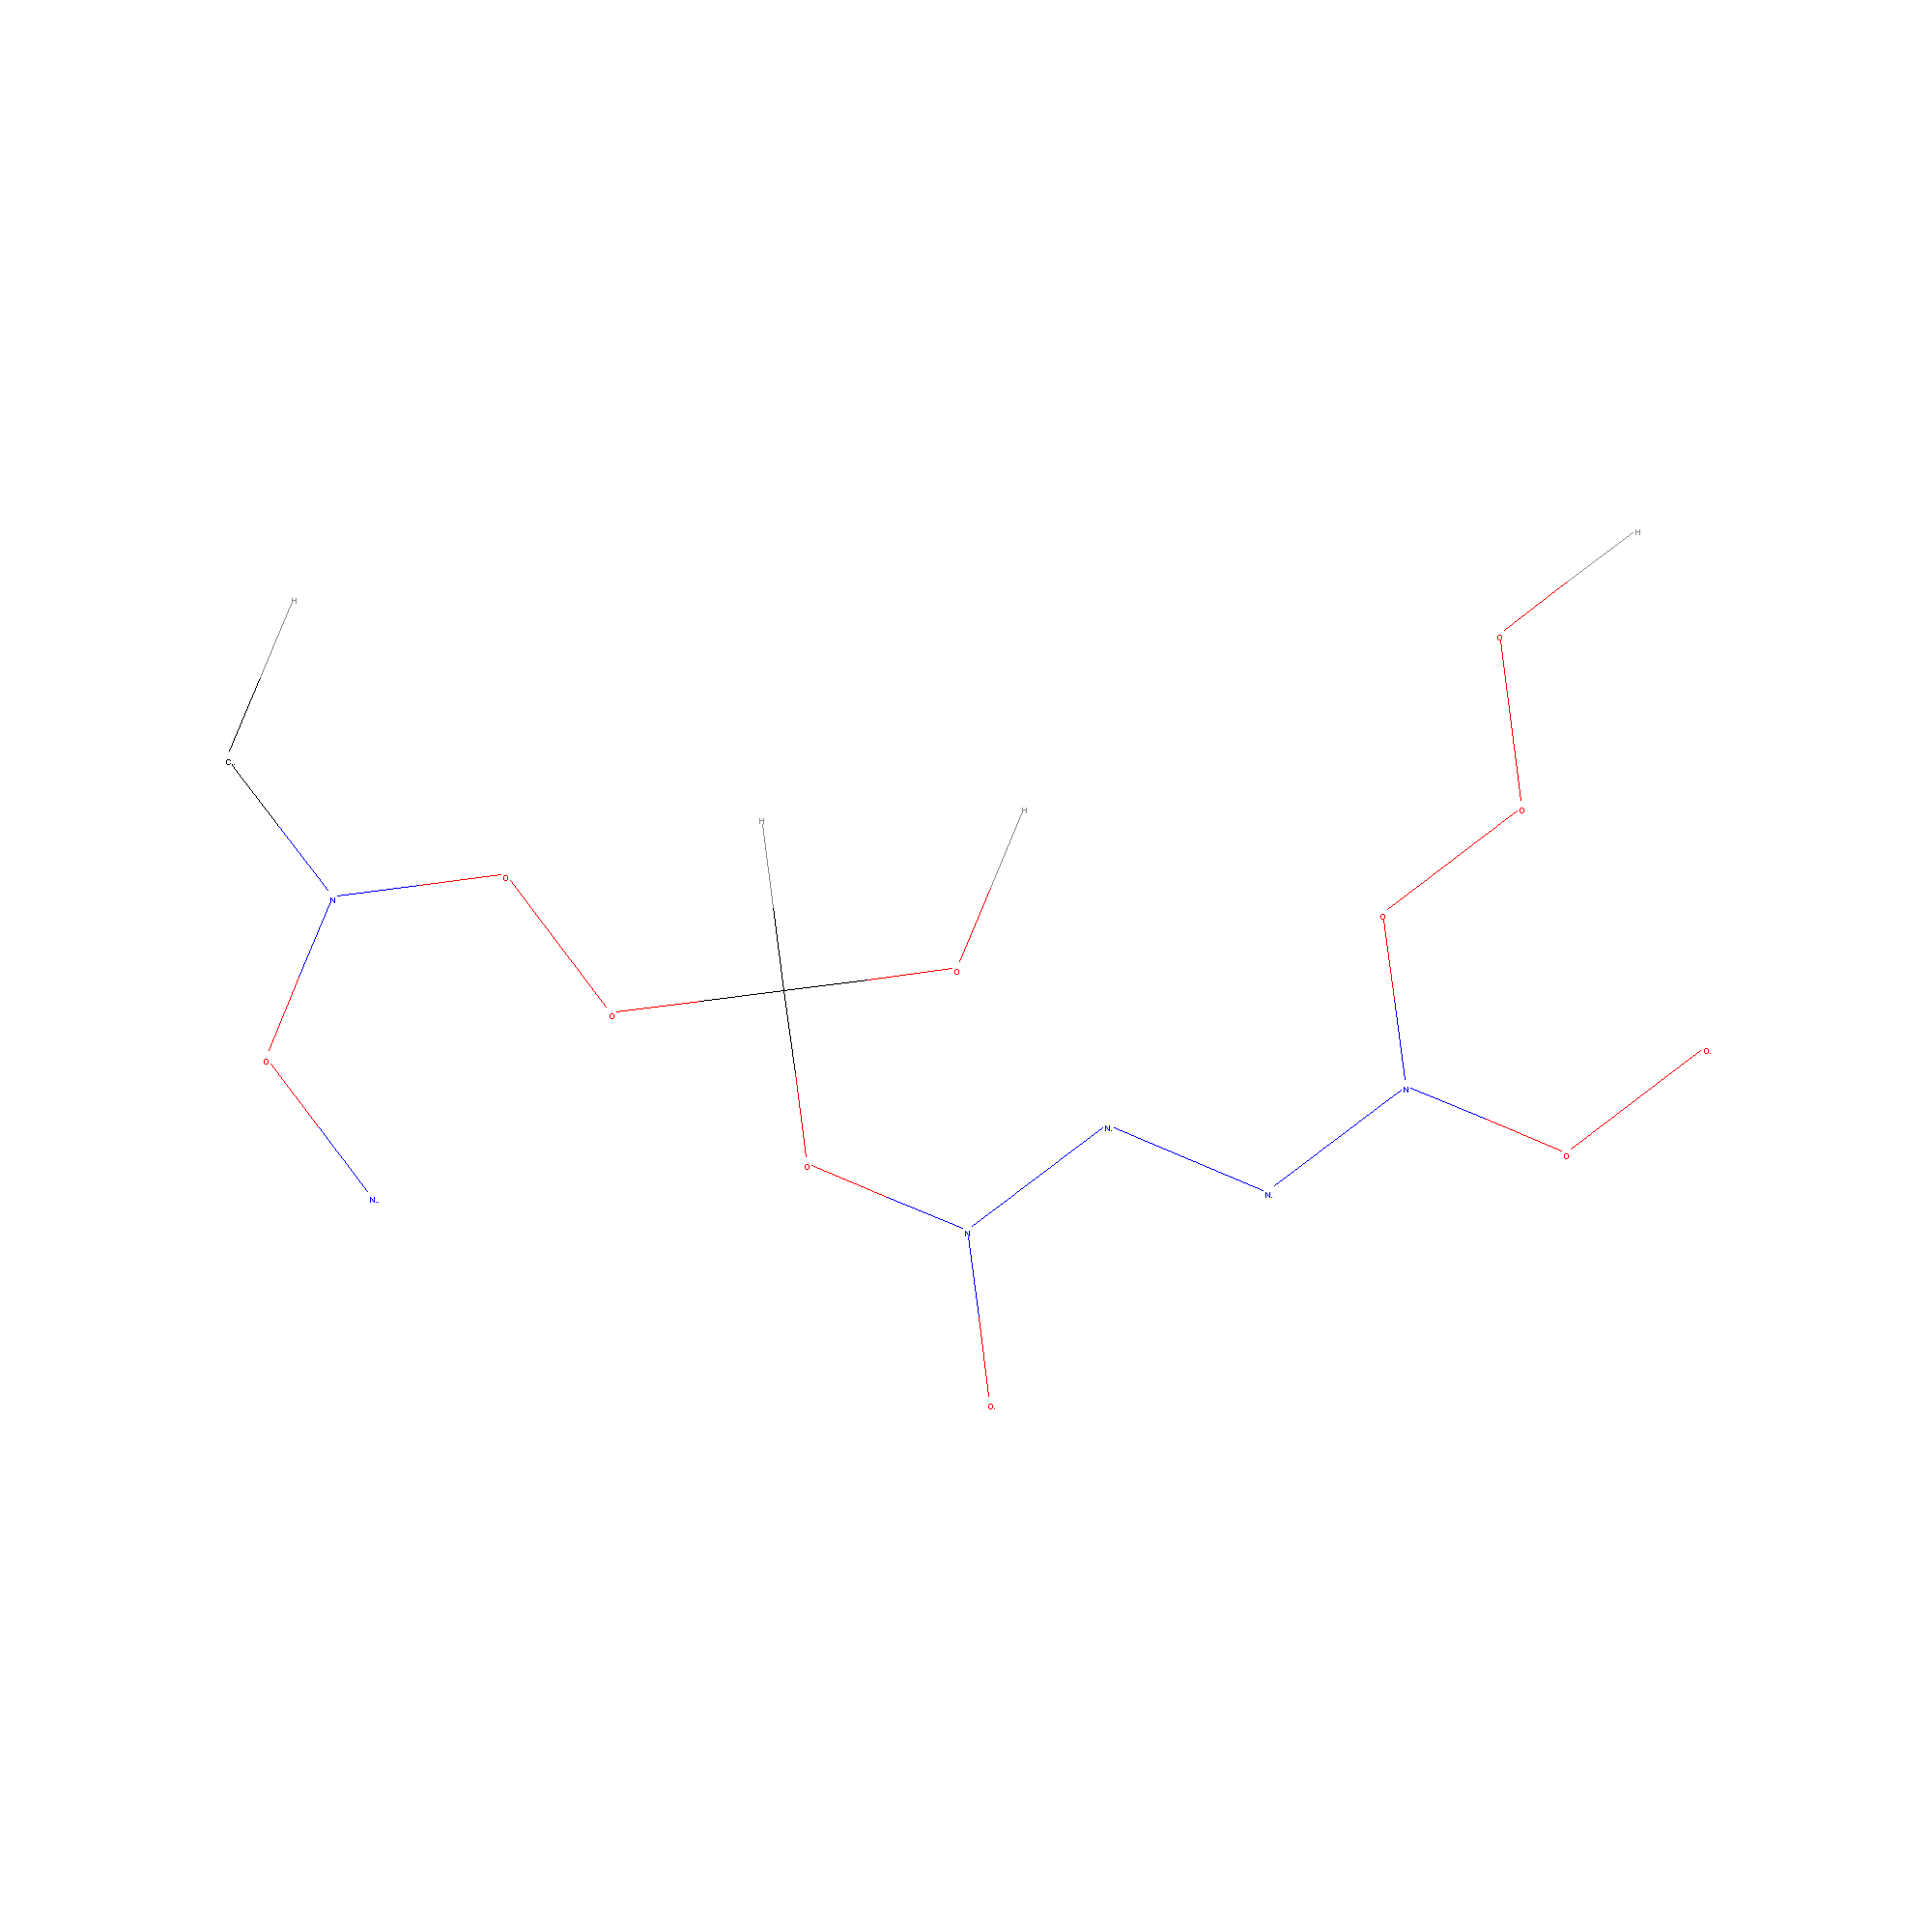
\includegraphics[width=0.45\linewidth]{figures/strategies-2-03-molecule.png}
	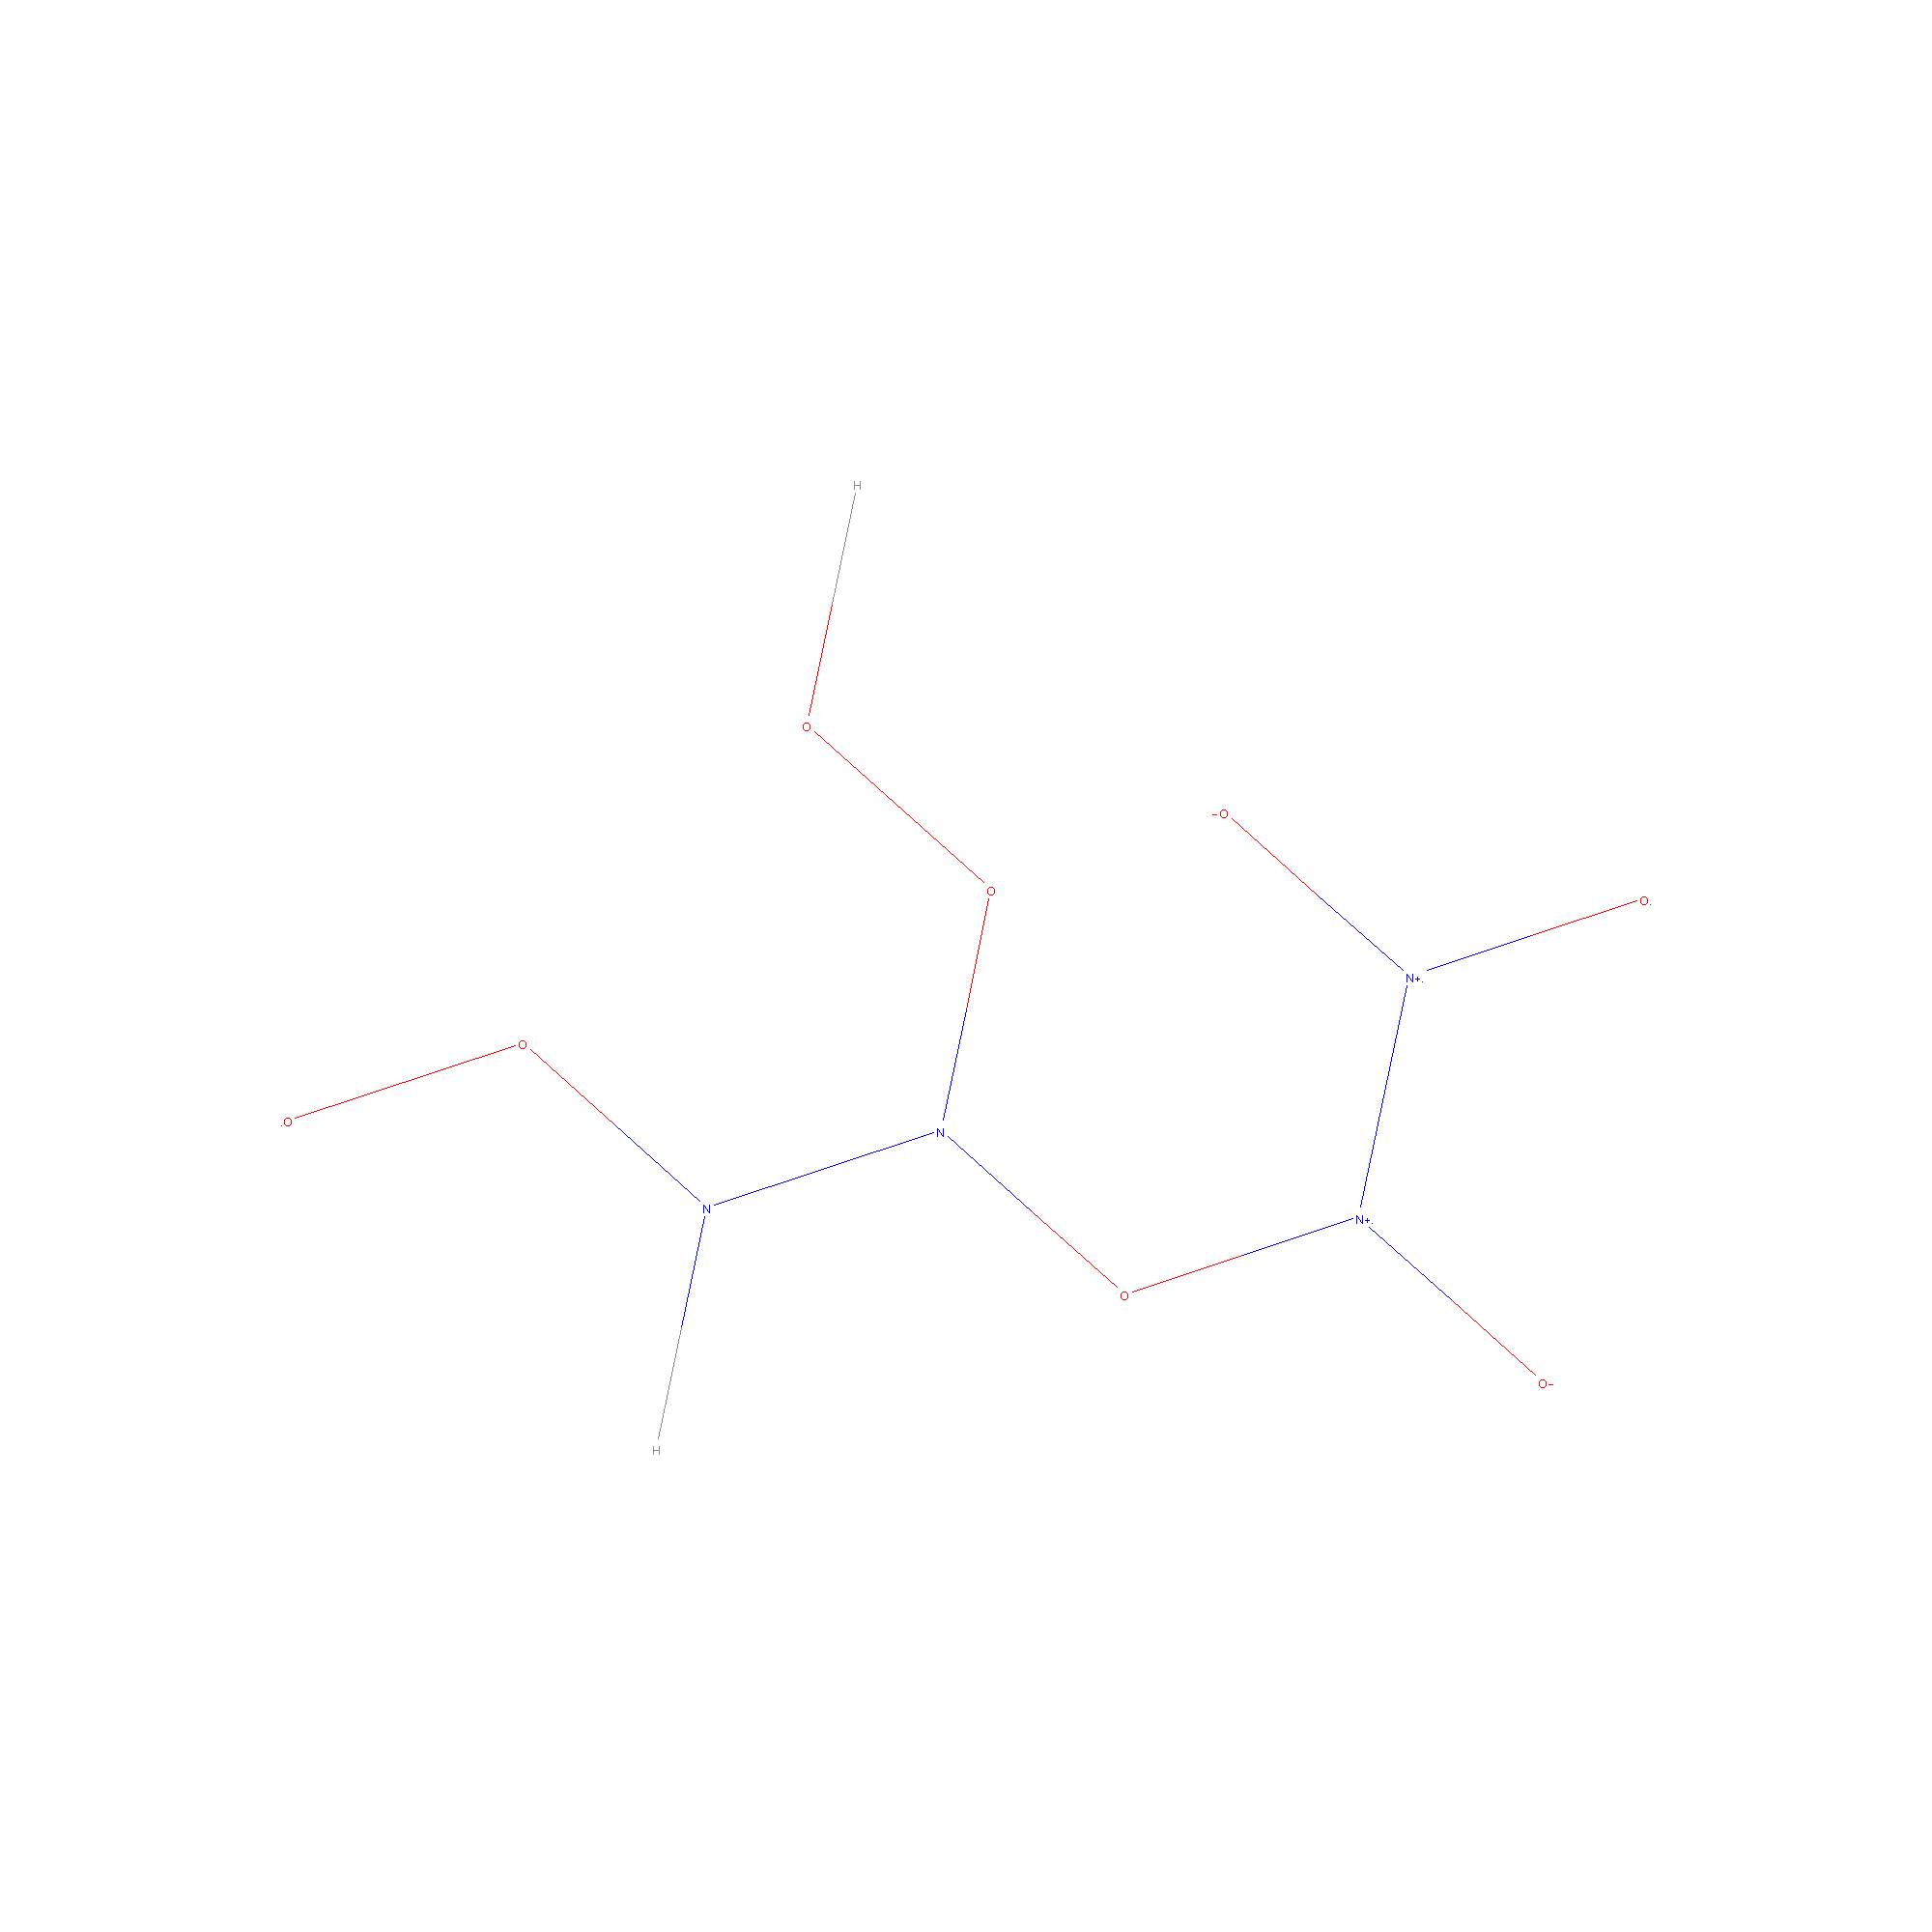
\includegraphics[width=0.45\linewidth]{figures/strategies-6-02-molecule.png}
	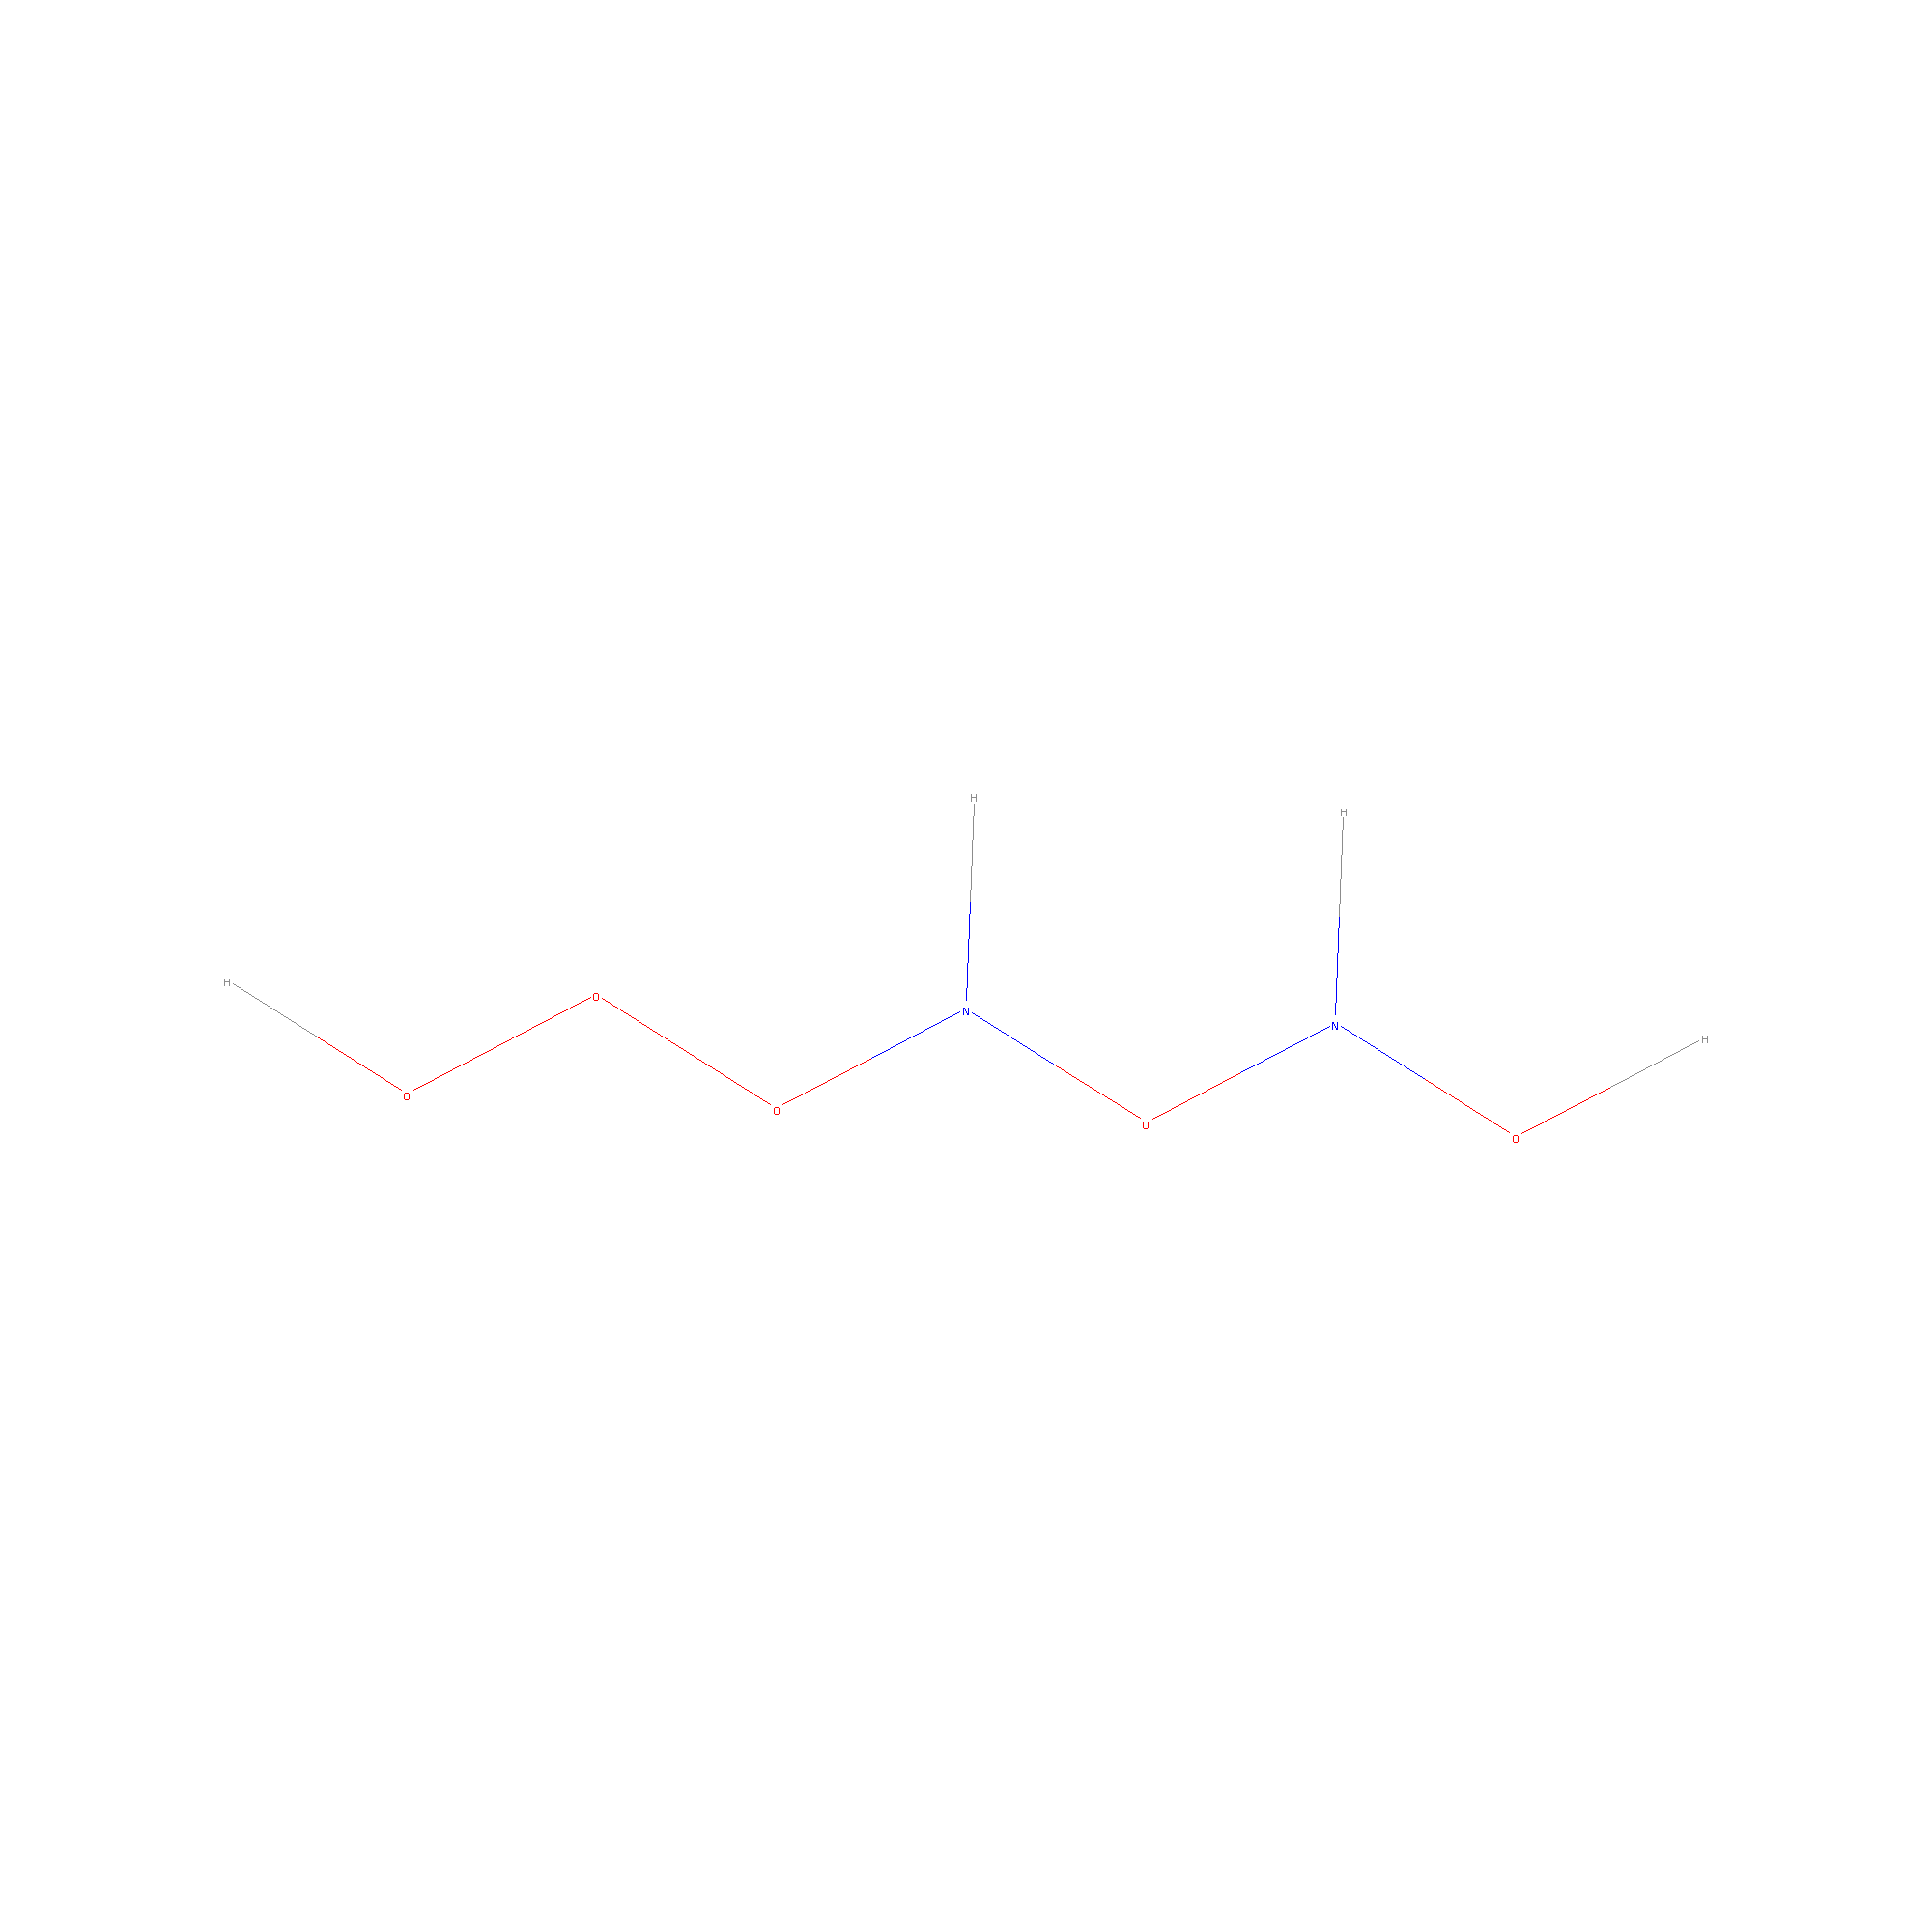
\includegraphics[width=0.45\linewidth]{figures/strategies-13-01-molecule.png}
	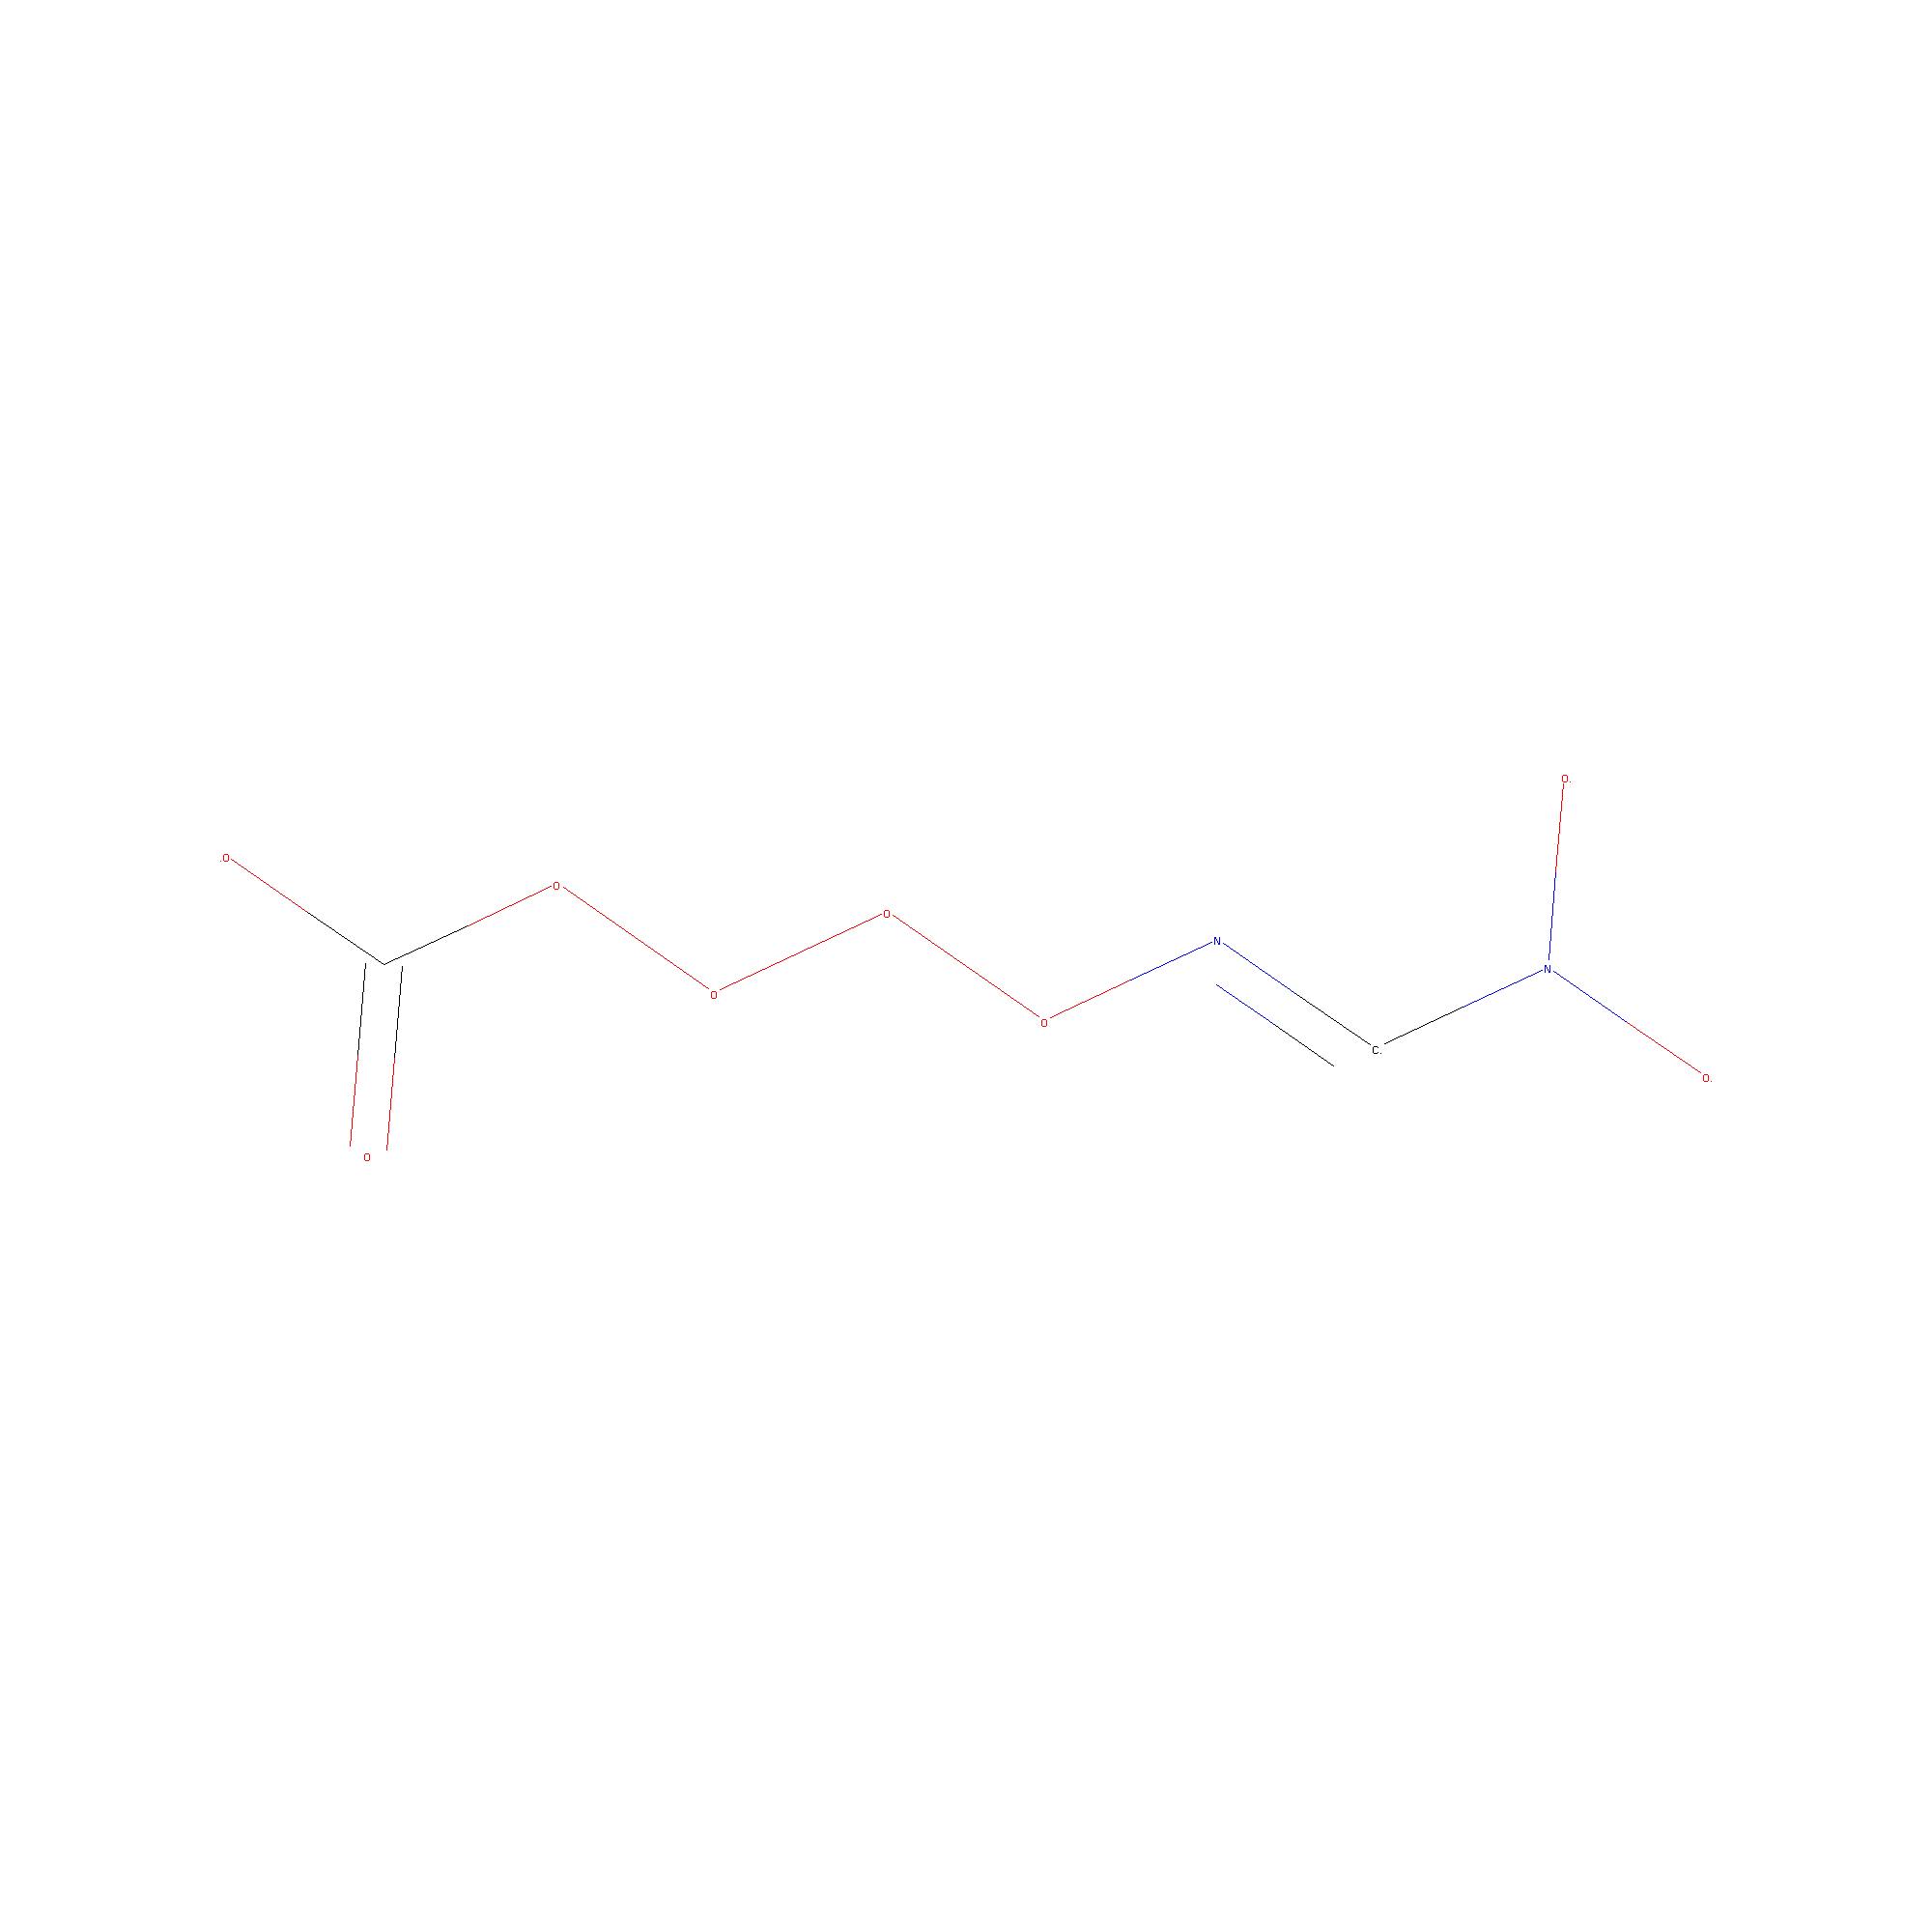
\includegraphics[width=0.45\linewidth]{figures/strategies-15-01-molecule.png}
	\caption[Example molecules generated by ToyWorld]{Example molecules generated by ToyWorld, rendered as 2-D objects from the original SMILES notation - [H][C]N(O[N])OOC([H])(O[H])ON([O])[N][N]N(O[O])OOO[H] (top left), [H]OON(O[N+]([O-])[N+]([O])[O-])N([H])O[O] (top right), [H]OOON([H])ON([H])O[H] (bottom left) and [O]C(=O)OOOON=[C]N([O])[O]  (bottom right)}\label{fig:toyworld-example-molecules}
\end{figure}

\section{Energy Model}\label{energy-model}

Energy within ToyWorld is found in only three standard forms -- kinetic,
internal and potential.

\begin{itemize}
	\item
 Kinetic energy is the energy of motion, and equals $\frac{1}{2}mv^2$
 where $m$ is the mass of a molecule and $v$ its velocity.
	\item
 Internal energy is an abstraction of vibrational energy or heat energy
 within a molecule. Internal energy, while incidentally consistent with
 real-world chemical models, is actually included in ToyWorld as a
 major mechanism to introduce stochasticity in reactions. Without
 internal energy, all excess energy following a reaction must be
 allocated to kinetic energy (following energy conservation), and so
 there is an iso-map between reaction and product kinetic energies.
 With internal energy, we can divert an arbitrary proportion into
 internal energy and therefore we have a stochastic multi-map.
	\item
 Potential energy is the energy associated with the bonds between
 Atoms. Creating a bond reduces the potential energy of a molecule;
 breaking a bond increases it. The potential energy of a molecule is
 the sum of the potential energies of every bond in the molecule. The
 base state of no bonds is equal to $0$, and so molecules with bonds
 have negative potential energy. The specific value of each bond is
 absolutely determined by the atomic number of the two Atoms at either
 end of the bond, and the type of bond itself -- single, double or
 triple. ToyWorld provides a table of standard values in
 \cref{default_bond_energies}, based upon real-world chemistry.
 Unspecified bonds are given the average energy of specified bonds of
 the same bond type. Examples of molecules with associated potential
 energies are given in \cref{example_potential_energies}.
\end{itemize}

Our energy model enforces conservation of mass so reactions can be
represented solely by bond changes in RDKit. This follows the approach
taken in graph-based chemistries such as GGL/ToyChem
\autocite{Benko2003,Benko2005} where reactions are modelled as a series
of changes to graph edges, or bonds, only.

\begin{table}[t]
	\begin{center}
		\caption[Average Bond Dissociation Enthalpies]{Average Bond Dissociation Enthalpies in kcal per mole -- source: \url{http://www.cem.msu.edu/~reusch/OrgPage/bndenrgy.htm}}\label{default_bond_energies}
		\begin{tabular}{@{}lp{2cm}p{2cm}p{2cm}@{}}
			\toprule
			Bond Type & Atom 1 & Atom 2 & Energy of both break and formation(simulation units) \\
			\midrule
			Single    & H      & H      & 104.2                                                \\
			Single    & C      & C      & 83                                                   \\
			Single    & N      & N      & 38.4                                                 \\
			Single    & O      & O      & 35                                                   \\
			Single    & H      & C      & 99                                                   \\
			Single    & H      & N      & 93                                                   \\
			Single    & H      & O      & 111                                                  \\
			Single    & C      & N      & 73                                                   \\
			Single    & C      & O      & 85.5                                                 \\
			Single    & N      & O      & 55                                                   \\
			Double    & C      & O      & 185                                                  \\
			Double    & C      & C      & 146                                                  \\
			Double    & N      & N      & 149                                                  \\
			Double    & O      & O      & 119                                                  \\
			Double    & C      & N      & 147                                                  \\
			Double    & N      & O      & 143                                                  \\
			Triple    & C      & O      & 258                                                  \\
			Triple    & C      & C      & 200                                                  \\
			Triple    & N      & N      & 226                                                  \\
			Triple    & C      & N      & 213                                                  \\
			Quadruple & C      & C      & 200                                                  \\
			\bottomrule
		\end{tabular}
	\end{center}
\end{table}

\begin{table}[t]
	\begin{center}
		\caption{Example potential energies calculated by the DefaultChemistry module using simplified bond energies}\label{example_potential_energies}
		\begin{tabular}{@{}p{3cm}p{5cm}p{2.5cm}@{}}
			\toprule
			Molecule   & SMILES                   & Potential Energy \\
			\midrule
			H$_2$O     & [H]O[H]                  & -222.0           \\
			H$_2$      & [H][H]                   & -104.2           \\
			O$_2$      & O=O                      & -119.0           \\
			N$_2$O$_4$ & [O-][N+](=O)[N+]([O-])=O & -434.4           \\
			NO$_2$     & N(=O)[O]                 & -198.0           \\
			\bottomrule
		\end{tabular}
	\end{center}
\end{table}%

\subsection{Energy transformations}\label{energy-transformations}

The only energy transformations that occur in ToyWorld are those that
occur during reactions. The energy at the beginning of the reaction is
fully bound in the potential, internal and kinetic energies of the
reactants. At the moment of collision, that portion of the kinetic
energy due to the collision (kinetic energies of reactants less kinetic
energy of centre of mass) is transformed into internal energy
in the combined reactants. If a bond forms in this phase
the freed potential energy is added into this pool of internal energy;
any bond that breaks transforms internal energy into increased potential
energy. Post-collision, a portion of the the pool of remaining internal
energy is transformed back into kinetic energy. The division may be all
to kinetic energy or all to internal or anywhere in between. All as
kinetic would represent a more elastic collision; if all remains as
internal energy, the collision is fully inelastic.

Reactions are modelled as head-on elastic collisions between two
reactants with changes to kinetic energy equalling the increase or
decrease in molecular potential energy associated with the creation,
destruction or change of order of bonds. Creation of a bond results in a
reduction of molecular potential energy and an increase to kinetic
energy; destruction results in the reverse. A change in bond type is
modelled as the sum of a bond creation and of a bond destruction. Total
energy in the system is always constant, and equal to the sum of the
initial kinetic energy of all molecules plus the sum of their potential
energies.

\begin{figure}[t]
	\begin{center}
		\begin{tikzpicture}
			[enode/.style={circle,draw=gray!50,inner sep=5pt,minimum size=30pt}]
			\node[enode] (pe) at (6,4) {Potential Energy (PE)};
			\node[enode] (ie) at (1,1) {Internal Energy (IE)};
			\node[enode] (ke) at (11,1) {Kinetic Energy (KE)};
		\end{tikzpicture}
		\caption{Energy transformations in ToyWorld}
		\label{fig:energy_transformations}
	\end{center}
\end{figure}

Reactions conserve energy, and hence the total energy in the reaction
vessel should be constant. However, energy can be explicitly added to
and removed from the system from outside. Either case is modelled as a
uniform change in all molecular internal energies (heat and vibration).
This changes the size of the pool from which the kinetic energies of the
product molecules are determined after a collision or reaction. Adding
energy to the system increases each molecule's internal energy, which
increases the size of the pool of merged internal and kinetic energies
on collision or reaction, which increases the likely kinetic energies of
the product molecules. Removing energy from the system has of course the
opposite affect, down to the point where effectively all motion and
hence all reaction activity ceases.

\section{Reactant and product selection strategies}\label{reactant-and-product-selection-strategies}

A reaction may be seen as two stages in sequence: first, the choice of reactants from a population of possible reactant molecules (the Reactant selection strategy, denoted here by $S_\mathrm{Reactant}$), and second, the determination of products given that set of reactants (Product selection strategy, denoted $S_\mathrm{Product}$). The total energy (that is, potential + kinetic + internal) of the system is maintained, as is the total momentum of the molecules.

\section{Reactant selection strategies: selecting reactants for a reaction}\label{reactant-selection-strategies}

\autocite{Faulconbridge2011} describes two generic strategies for the
selection of reactants -- spatial and aspatial -- where the primary
difference is whether molecular position is a factor in reactant
selection. It is possible to further generalise this scheme by
considering other differentiating factors. Analogous with real-world
chemistry, a cumulative scheme presents itself starting with the pure
aspatial, or uniform probability strategy, and then proceeding through
the spatial strategy, based on molecular kinetics, to kinetics plus
intra-molecular and external forces such as electromagnetism. These
strategies can be viewed as being based on increasing derivatives of
position or location in the reaction vessel; from no position (uniform
selection), through fixed position (uninteresting as we cannot have a
sequence of reactions without motion) to the first derivative (velocity
or kinetic selection) and finally to the second derivative
(acceleration, or force selection.) Accordingly we adopt this more
detailed classification for the descriptions below.

\subsection{Uniform selection}\label{uniform-selection}

In a uniform selection strategy ($S_\mathrm{Reactant} = \mathrm{Uniform}$), reactants are chosen at random with equal (uniform) probability from the population: no property of a molecule has an effect on the selection. Conceptually we have a well-stirred reaction container with no intra-molecular forces.

\subsection{Kinetic selection.}\label{kinetic-selection.}

By contrast, in a kinetic selection strategy ($S_\mathrm{Reactant} = \mathrm{Kinetic}$) molecules have spatial position (and implicitly, velocity) within some assumed reaction vessel, and selection is determined by molecular position -- molecules which are spatially co-located (that is, in collision) form a reactant set. Molecules move at constant velocity until they collide with something else (either another molecule or possibly a boundary of an explicit reaction vessel) and then either react, or bounce.  Currently in our work we assume that all molecules have a fixed and common size and shape (circular in two-dimensions), irrespective of molecular formula.

\subsection{Intra-molecular selection and external force selection}\label{intra-molecular-selection-and-external-force-selection}

More complicated forms, where molecular velocities are not constant, can
be generated by the introduction of some combination of intra-molecular
forces (such as electromagnetism) or external forces (such as gravity or
heat.)

\section{Product selection strategies: determining the products of a
reaction}\label{product-selection-strategies}

In the ToyWorld chemical model, all reactions arise solely from the
properties of the reacting molecules: it therefore defines a
\emph{strongly constructive} chemistry in the sense defined earlier. As
ToyWorld enforces conservation of mass, reactions can be represented
solely by bond changes. This is closely related conceptually to
graph-based chemistries such as GGL/ToyChem
\autocite{Benko2005,Benko2003}, RBN-World \autocite{Faulconbridge2011}
or NAC \autocite{Suzuki2006} where reactions are modelled as a series of
changes to graph edges. However, in ToyWorld, and RDKit, the graph is
implicit rather than explicit as it is in a graph-based chemistry.

For each interaction between two molecules we generate a list of reaction alternatives by enumerating all possible single bond additions, bond subtractions, and changes in bond type between the reactants. Each alternative is the result of a single one of these changes. For example, the reactants H\textsubscript{2} and O\textsubscript{2} generate three reaction alternatives: breaking of the H-H bond, breaking of the O=O double bond, and a transformation of the O=O double bond to a single bond. The reactants H\textsuperscript{+} and OH\textsuperscript{-} give two alternative reactions: breaking of the O-H bond (giving H+H\textsuperscript{+}+O\textsuperscript{-}) and formation of a single bond between H\textsuperscript{+} and O to give H\textsubscript{2}O. We restrict the options to those that can be generated by a single change to the bond structure of the reactants.

Each reaction alternative therefore can be completely described by the
pair of the products of the reaction (that result from the single bond
addition, subtraction or change) and the associated change in overall
potential energy, which of course will be the same as the potential
energy change of the single bond alteration.

Creation of a bond results in a reduction of molecular potential energy,
while bond destruction results in an increase. A change in bond type is
equivalent to a creation and then a destruction. The magnitude of the
change in potential energy, measured in arbitrary energy units, is taken
from a table of bond energies for each combination of atoms and bond
type (\cref{default_bond_energies}. The standard table is based upon
a simplification of real-world chemical bond energies. For example, the
creation of a H-H bond releases 104.2 units; the breaking of a C=O
double bond takes 185 energy units. \cref{example_potential_energies}
shows the potential energy for a sample of molecules.

How should we choose between alternative sets of possible products for
the same reactants? Various product strategies appear plausible: the
random choice of an alternative; the most complex alternative; least
complex; rarest; most common, and so on, but each strategy requires
effort to develop and evaluate.

We also consider a strategy with minimal bias: a Uniform selection
strategy ($S_\mathrm{Product} = \mathrm{Uniform}$), where every
alternative product set has equal probability of selection.

\subsection{Least Energy Strategy}\label{least-energy-strategy}

When following a Least Energy strategy
($S_\mathrm{Product} = \mathrm{LeastEnergy}$) we select a reaction by
choosing with uniform probability from a distribution of reaction
alternatives weighted by the total of the energy changes associated with
the bond changes. This biases selection towards the Least Energy
alternative; the strength of the bias is determined by the degree of the
weighting. \cref{fig1} shows an example of the shift in products that occurs as a result of
this weighting as the overall quantity of energy in the system is
changed.

Specifically, let $E_i$ denote the energy required for the bond change in the reaction option. If $E_i > 0$ the reaction is exothermic, or releases energy; otherwise it is endothermic, requiring energy to proceed.

We calculate a weighted value, $e_i$, based on the combination of $E_i$ and the available energy for the reaction, $E_{avail} > 0$, as follows:

\begin{displaymath}
	e_i=
	\begin{cases}
		\lvert E_i\rvert, & (1) \text{  if $E_i < 0$;}         \\
		0,                & (2) \text{  if $E_{avail} < E_i$;} \\
		E_{avail}--E_i,   & (3) \text{  otherwise.}            
	\end{cases}
\end{displaymath}\label{weighting-calculation}

Then, for reaction option $i$ of $n$ options, $p_i = e_i / \sum\limits_{i=1}^n e_i$, where $p_i$ is the probability of option $i$ being selected. A number is chosen from the uniform distribution $[0,1]$ and the selected reaction is found from the inverse of the CDF given by $p_i\text{ for all }i$ by searching for the reaction at that point in the CDF. This method has the property that the probability of a reaction being selected is proportional to its weight.

As a result, for exothermic reactions, highly exothermic reactions are preferred to slightly exothermic ones. For endothermic reactions, the available energy must exceed the energy required by the reaction, and the reaction is preferred according to the degree of the surplus. Note that an option where the energy required exceeds that available ($E_{avail} < E_i$) will have $p_i = 0$, and hence can not be selected. This behaviour is shown in \cref{fig:reaction_selection_weights}.

\begin{figure}[t]
	\begin{center}
		\begin{tikzpicture}
			[enode/.style={circle,draw=gray!50,fill=white,radius=0.5cm}]
			\pgftext[at=\pgfpoint{2cm}{0cm},left,base]{\pgfimage[width=0.5\linewidth]{figures/reaction_selection_weights}};
			\node[enode] at (5.5,6) {1};
			\node[enode] at (7,4) {2};
			\node[enode] at (8,3.2) {3};
		\end{tikzpicture}
		\caption{Weighting calculation for reaction selection under a Least Energy Strategy. Numerical labels refer to cases in \cref{weighting-calculation}.}\label{fig:reaction_selection_weights}
	\end{center}
\end{figure}

\subsection{Energy transformations during a reaction}\label{energy-transformations-during-a-reaction}

Molecules have kinetic energy; when they collide the form of the
interaction follows from the energy transformations between kinetic and
internal and potential energy that are preferred under the chemical
model; and finally, the trajectory taken by the resulting products of
the interaction is given by their final post-collision kinetic energy.

First, we determine the kinetic energy of the centre of mass of the
reactants. The available energy to drive the reaction is the total
kinetic energy of the reactants plus the internal energy of the
reactants less the kinetic energy of the centre of mass.

Consider the case where two particles of equal mass but opposite
velocity collide. The KE of the centre of mass will be zero (as it is
motionless) and the energy liberated by the collision will be the sum of
the kinetic and internal energies of the particles.

At the other extreme, consider two equal mass particles, travelling with
the same velocities. Intuitively, it is obvious that the only energy
released by their infinitesimally gentle collision is from their
internal energies, and this is confirmed by the calculation where the
kinetic energy of the centre of mass will equal the combined kinetic
energies of the reactants, leaving only the combined internal energies.

The available energy for bond modifications is calculated as the sum of
the kinetic energies of the reactants less the energy of their centre of
mass, plus any energies internal to the reactants. The final kinetic
energies of the products equals the sum of the initial kinetic energies
of reactants less the change in molecular potential energy from bond
changes and the change in internal energies. Total energy in the system
is always constant, and equal to the sum of the initial kinetic energy
of all molecules plus the sum of their potential energies and internal
energies.

The Reactor Algorithm selects one of the reaction alternatives by
choosing from a distribution of reaction alternatives weighted by
associated energy changes (as discussed in
\cref{product-selection-strategies}.)

\subsection{Setting product velocities and internal energies}\label{setting-product-velocities-and-internal-energies}

The final step in the reaction mechanism is to determine the velocities
and internal energies of the reaction products following the reaction.
Although the method is standard physics, there are two complications:
the number of products may or may not be the same as the number of
reactants, and the pre-reaction energy and post-reaction energy vary as
the reaction itself either consumes or liberates energy.

The only constraints are that velocities of the product molecules must
conserve momentum and total energy within the reacting system. We
recognize that within the frame of reference of the centre of momentum
of the reacting system, the vector sum of the momentum of the products
must equal zero. Therefore one possible solution to the product
velocities is to arrange their vector momentums according to simple
geometry: for two products, we arrange their momentums in a line (line
\cref{alg:2products} in \cref{alg:post_collision_adjustments}); for three
products, an equilateral triangle (line \cref{alg:3products}), and by
extension, for four products, a square and so on.

\begin{algorithm}
	\KwData{Reactant molecules fully specified with energies and velocities, Product molecules without energies or velocities}
	\KwResult{Velocities for each Product molecule and total Internal Energy for all Product molecules $\ni$ total energy and momentum conserved}
	%$\text{sum of reactant kinetic energies}\leftarrow \sum\limits_{i=1}^n \text{kinetic energy}_i$\;
	%$\text{sum of reactant internal energies}\leftarrow \sum\limits_{i=1}^n \text{internal energy}_i$\;
	$\text{kinetic energy of CoM}\leftarrow \frac{1}{2}(\text{sum of reactant masses})(\text{velocity of CoM})^2$\;
	\BlankLine
	$\text{collision energy}\leftarrow \text{sum of reactant kinetic energies}+\text{sum of reactant internal energies}-\text{kinetic energy of CoM}$\;
	\BlankLine
	\For(\tcp*[f]{Transform into CoM frame}){$i\leftarrow 1$ \KwTo $\text{number of Products}$}{\label{alg:lab_to_CoM_frame}
		$v^\prime_i\leftarrow v_i-\text{CoM velocity}$\;
	}
	\BlankLine
	\uIf(\tcp*[f]{Conservation of momentum implies all excess energy must go into internal energy}){Number of products = 1}{\label{alg:allocate_energies}
		$\text{Internal energy of Products}\leftarrow \text{collision energy}$\;
	}
	\uElse{
		$\text{ke}\leftarrow \text{random}([0,1])$\;
		$\text{Internal energy of Products}\leftarrow \text{collision energy}-\text{ke}$\;
	}
	\BlankLine
	\Switch(\tcp*[f]{Find a set of momentum vectors that sum to zero...}){Number of products}{
		\uCase(\tcp*[f]{One product}){1}{
			$mv^\prime\leftarrow (0,0,0)$\;
		}
		\uCase(\tcp*[f]{Two products}){2}{\label{alg:2products}
			$mv\leftarrow 2\text{ke}\prod\limits_{i=1}^n \text{mass}_i/\sum\limits_{i=1}^n \text{mass}_i$\;
			$mv^\prime_1\leftarrow (v^\prime_{i\theta}+\frac{\pi}{2},v^\prime_{i\rho}+\frac{\pi}{2},mv)$\;
			$mv^\prime_2\leftarrow (v^\prime_{i\theta}+\frac{3\pi}{2},v^\prime_{i\rho}+\frac{3\pi}{2},mv)$\;
		}
		\uCase(\tcp*[f]{Three products}){3}{\label{alg:3products}
			$mv\leftarrow 2\text{ke}\prod\limits_{i=1}^n \text{mass}_i/\sum\limits_{i=1}^n \text{mass}_i$\;
			$mv^\prime_1\leftarrow (v^\prime_{i\theta}+\frac{\pi}{3},0,mv)$\;
			$mv^\prime_2\leftarrow (v^\prime_{i\theta}-\frac{\pi}{3},0,mv)$\;
			$mv^\prime_3\leftarrow (v^\prime_{i\theta}-\pi,0,mv)$\;
		}
	}
	\BlankLine
	\For(\tcp*[f]{Convert momentums to velocities...}){$i\leftarrow 1$ \KwTo $\text{number of products}$}{
		$v^\prime_i\leftarrow mv^\prime_i / \text{mass}_i$\;
	}
	\BlankLine
	\For(\tcp*[f]{Transform back to standard frame}){$i\leftarrow 1$ \KwTo $\text{number of products}$}{\label{alg:CoM_to_lab_frame}
		$v_i\leftarrow v^\prime_i+\text{CoM velocity}$\;
	}
	\caption{Algorithm to set post-collision velocities and internal energies}\label{alg:post_collision_adjustments}
\end{algorithm}


Following a standard method, we first transfer the molecules from the
frame of reference of the reaction vessel into the centre of mass (CoM)
reference frame by subtracting the velocity of the CoM from each
particle (line \cref{alg:lab_to_CoM_frame}). Correspondingly, we also
adjust the energy of the collision by subtracting the KE of the CoM. We
recognize that in the CoM frame the vector sum of the momentums will be
zero; working in this frame reduces the number of vectors we must sum by
one (the momentum of the CoM itself.)

We then arbitrarily choose the proportion of total available energy to allocate to the product kinetic energies and assign the remainder to internal energy (line \cref{alg:allocate_energies}.) From the kinetic energy allocation we can determine the total scalar momentum of the products using $KE = 0.5 * velocity * momentum$, and arrange the vector momentums according to the geometry described earlier.

Finally, we convert from the CoM reference frame to the initial frame by
adding back the velocity of the CoM (line \cref{alg:CoM_to_lab_frame}).

This method satisfies our requirements of conservation of momentum and
energy for arbitrary numbers of reactants and products while being
computationally straightforward. The limitation is that product vectors
are arranged in regular and consistent, although reasonably realistic,
configurations. An improvement would be to perturb the geometry of the
vectors in the CoM frame to remove the regularity.

The outcomes for each reaction alternative from an example collision are
shown in \cref{fig:collision_diagrams}.

\tdplotsetmaincoords{60}{110}

\begin{figure}
	\centering
	\subcaptionbox{O=C=O + C$\rightarrow$ [O] + C + [C]=O}[0.5\textwidth]{%
		\begin{tikzpicture}[scale=3,tdplot_main_coords]
			\coordinate (O) at (0,0,0);
			\draw[thick,->] (0,0,0) -- (1,0,0) node[anchor=north east]{$x$};
			\draw[thick,->] (0,0,0) -- (0,1,0) node[anchor=north west]{$y$};
			\draw[thick,->] (0,0,0) -- (0,0,1) node[anchor=south]{$z$};
			\node at (1,1,0) {};
			\tdplotsetcoord{CM0}{0.545078574376}{-35.9326309999}{-145.082834065};\tdplotsetcoord{CM1}{-0.545078574376}{-35.9326309999}{-145.082834065};
			\draw[color=black,densely dotted,-stealth] (CM0)-- (CM1);\tdplotsetcoord{I0}{-0.741455902351}{53.4742770534}{-140.637846457};
			\tdplotsetcoord{I1}{-1.00269224405}{-269.549896905}{-273.397556374};
			\draw[color=red,-stealth] (I0) node[font=\tiny,color=black]{O=C=O}-- (O);
			\draw[color=red,-stealth] (I1) node[font=\tiny,color=black]{[H]C([H])([H])[H]}-- (O);
			\draw[dotted, color=black] (O) -- (I0xy); \draw[dotted, color=black] (I0) -- (I0xy);
			\draw[dotted, color=black] (O) -- (I1xy); \draw[dotted, color=black] (I1) -- (I1xy);
			\tdplotsetcoord{O0}{0.791487199406}{-24.6589855625}{-70.1992043245};
			\tdplotsetcoord{O1}{0.790684881135}{-24.6841653158}{-219.830383842};
			\tdplotsetcoord{O2}{0.342756745318}{-57.7497471497}{-145.082834065};
			\draw[color=blue,-stealth] (O) -- (O0) node[font=\tiny,color=black]{[O]};
			\draw[color=blue,-stealth] (O) -- (O1) node[font=\tiny,color=black]{[H]C([H])([H])[H]};
			\draw[color=blue,-stealth] (O) -- (O2) node[font=\tiny,color=black]{[C]=O};
			\draw[dotted, color=black] (O) -- (O0xy); \draw[dotted, color=black] (O0) -- (O0xy);
			\draw[dotted, color=black] (O) -- (O1xy); \draw[dotted, color=black] (O1) -- (O1xy);
			\draw[dotted, color=black] (O) -- (O2xy); \draw[dotted, color=black] (O2) -- (O2xy);
		\end{tikzpicture}}%
	\subcaptionbox{O=C=O + C$\rightarrow$ C + [O][C]=O}[0.5\textwidth]{%
		\begin{tikzpicture}[scale=3,tdplot_main_coords]
			\coordinate (O) at (0,0,0);
			\draw[thick,->] (0,0,0) -- (1,0,0) node[anchor=north east]{$x$};
			\draw[thick,->] (0,0,0) -- (0,1,0) node[anchor=north west]{$y$};
			\draw[thick,->] (0,0,0) -- (0,0,1) node[anchor=south]{$z$};
			\node at (1,1,0) {};
			\tdplotsetcoord{CM0}{0.545078574376}{-35.9326309999}{-145.082834065};\tdplotsetcoord{CM1}{-0.545078574376}{-35.9326309999}{-145.082834065};
			\draw[color=black,densely dotted,-stealth] (CM0)-- (CM1);\tdplotsetcoord{I0}{-0.741455902351}{53.4742770534}{-140.637846457};
			\tdplotsetcoord{I1}{-1.00269224405}{-269.549896905}{-273.397556374};
			\draw[color=red,-stealth] (I0) node[font=\tiny,color=black]{O=C=O}-- (O);
			\draw[color=red,-stealth] (I1) node[font=\tiny,color=black]{[H]C([H])([H])[H]}-- (O);
			\draw[dotted, color=black] (O) -- (I0xy); \draw[dotted, color=black] (I0) -- (I0xy);
			\draw[dotted, color=black] (O) -- (I1xy); \draw[dotted, color=black] (I1) -- (I1xy);
			\tdplotsetcoord{O0}{0.964870972861}{170.402519717}{-86.502709589};
			\tdplotsetcoord{O1}{0.690770768471}{-121.920061352}{-167.114195829};
			\draw[color=blue,-stealth] (O) -- (O0) node[font=\tiny,color=black]{[H]C([H])([H])[H]};
			\draw[color=blue,-stealth] (O) -- (O1) node[font=\tiny,color=black]{[O][C]=O};
			\draw[dotted, color=black] (O) -- (O0xy); \draw[dotted, color=black] (O0) -- (O0xy);
			\draw[dotted, color=black] (O) -- (O1xy); \draw[dotted, color=black] (O1) -- (O1xy);
		\end{tikzpicture}}%
\end{figure}\begin{figure}
\centering
\subcaptionbox{O=C=O + C$\rightarrow$ [O] + C + [C]=O}[0.5\textwidth][l]{%
	\begin{tikzpicture}[scale=3,tdplot_main_coords]
		\coordinate (O) at (0,0,0);
		\draw[thick,->] (0,0,0) -- (1,0,0) node[anchor=north east]{$x$};
		\draw[thick,->] (0,0,0) -- (0,1,0) node[anchor=north west]{$y$};
		\draw[thick,->] (0,0,0) -- (0,0,1) node[anchor=south]{$z$};
		\node at (1,1,0) {};
		\tdplotsetcoord{CM0}{0.545078574376}{-35.9326309999}{-145.082834065};\tdplotsetcoord{CM1}{-0.545078574376}{-35.9326309999}{-145.082834065};
		\draw[color=black,densely dotted,-stealth] (CM0)-- (CM1);\tdplotsetcoord{I0}{-0.741455902351}{53.4742770534}{-140.637846457};
		\tdplotsetcoord{I1}{-1.00269224405}{-269.549896905}{-273.397556374};
		\draw[color=red,-stealth] (I0) node[font=\tiny,color=black]{O=C=O}-- (O);
		\draw[color=red,-stealth] (I1) node[font=\tiny,color=black]{[H]C([H])([H])[H]}-- (O);
		\draw[dotted, color=black] (O) -- (I0xy); \draw[dotted, color=black] (I0) -- (I0xy);
		\draw[dotted, color=black] (O) -- (I1xy); \draw[dotted, color=black] (I1) -- (I1xy);
		\tdplotsetcoord{O0}{0.95444795957}{-20.4286793523}{-48.3296764651};
		\tdplotsetcoord{O1}{0.953114678315}{-20.4573799628}{-241.693389093};
		\tdplotsetcoord{O2}{0.239763118095}{-84.1834478971}{-145.082834065};
		\draw[color=blue,-stealth] (O) -- (O0) node[font=\tiny,color=black]{[O]};
		\draw[color=blue,-stealth] (O) -- (O1) node[font=\tiny,color=black]{[H]C([H])([H])[H]};
		\draw[color=blue,-stealth] (O) -- (O2) node[font=\tiny,color=black]{[C]=O};
		\draw[dotted, color=black] (O) -- (O0xy); \draw[dotted, color=black] (O0) -- (O0xy);
		\draw[dotted, color=black] (O) -- (O1xy); \draw[dotted, color=black] (O1) -- (O1xy);
		\draw[dotted, color=black] (O) -- (O2xy); \draw[dotted, color=black] (O2) -- (O2xy);
	\end{tikzpicture}}%
\subcaptionbox{O=C=O + C$\rightarrow$ C + [O][C]=O}[0.5\textwidth][r]{%
	\begin{tikzpicture}[scale=3,tdplot_main_coords]
		\coordinate (O) at (0,0,0);
		\draw[thick,->] (0,0,0) -- (1,0,0) node[anchor=north east]{$x$};
		\draw[thick,->] (0,0,0) -- (0,1,0) node[anchor=north west]{$y$};
		\draw[thick,->] (0,0,0) -- (0,0,1) node[anchor=south]{$z$};
		\node at (1,1,0) {};
		\tdplotsetcoord{CM0}{0.545078574376}{-35.9326309999}{-145.082834065};\tdplotsetcoord{CM1}{-0.545078574376}{-35.9326309999}{-145.082834065};
		\draw[color=black,densely dotted,-stealth] (CM0)-- (CM1);\tdplotsetcoord{I0}{-0.741455902351}{53.4742770534}{-140.637846457};
		\tdplotsetcoord{I1}{-1.00269224405}{-269.549896905}{-273.397556374};
		\draw[color=red,-stealth] (I0) node[font=\tiny,color=black]{O=C=O}-- (O);
		\draw[color=red,-stealth] (I1) node[font=\tiny,color=black]{[H]C([H])([H])[H]}-- (O);
		\draw[dotted, color=black] (O) -- (I0xy); \draw[dotted, color=black] (I0) -- (I0xy);
		\draw[dotted, color=black] (O) -- (I1xy); \draw[dotted, color=black] (I1) -- (I1xy);
		\tdplotsetcoord{O0}{0.683938755498}{116.950434333}{-109.96313961};
		\tdplotsetcoord{O1}{0.613112203007}{-91.4698581679}{-158.027937122};
		\draw[color=blue,-stealth] (O) -- (O0) node[font=\tiny,color=black]{[H]C([H])([H])[H]};
		\draw[color=blue,-stealth] (O) -- (O1) node[font=\tiny,color=black]{[O][C]=O};
		\draw[dotted, color=black] (O) -- (O0xy); \draw[dotted, color=black] (O0) -- (O0xy);
		\draw[dotted, color=black] (O) -- (O1xy); \draw[dotted, color=black] (O1) -- (O1xy);
	\end{tikzpicture}}%
\end{figure}\begin{figure}
\centering
\subcaptionbox{O=C=O + C$\rightarrow$ [H] + [CH3] + O=C=O}[0.5\textwidth]{%
	\begin{tikzpicture}[scale=3,tdplot_main_coords]
		\coordinate (O) at (0,0,0);
		\draw[thick,->] (0,0,0) -- (1,0,0) node[anchor=north east]{$x$};
		\draw[thick,->] (0,0,0) -- (0,1,0) node[anchor=north west]{$y$};
		\draw[thick,->] (0,0,0) -- (0,0,1) node[anchor=south]{$z$};
		\node at (1,1,0) {};
		\tdplotsetcoord{CM0}{0.13448625105}{-35.9326309999}{-145.082834065};\tdplotsetcoord{CM1}{-0.13448625105}{-35.9326309999}{-145.082834065};
		\draw[color=black,densely dotted,-stealth] (CM0)-- (CM1);\tdplotsetcoord{I0}{-0.182938074093}{53.4742770534}{-140.637846457};
		\tdplotsetcoord{I1}{-0.247392444315}{-269.549896905}{-273.397556374};
		\draw[color=red,-stealth] (I0) node[font=\tiny,color=black]{O=C=O}-- (O);
		\draw[color=red,-stealth] (I1) node[font=\tiny,color=black]{[H]C([H])([H])[H]}-- (O);
		\draw[dotted, color=black] (O) -- (I0xy); \draw[dotted, color=black] (I0) -- (I0xy);
		\draw[dotted, color=black] (O) -- (I1xy); \draw[dotted, color=black] (I1) -- (I1xy);
		\tdplotsetcoord{O0}{1.0085637103}{-4.76020744144}{22.9882733079};
		\tdplotsetcoord{O1}{0.174049248064}{-27.6898552083}{-202.938127977};
		\tdplotsetcoord{O2}{0.113557100128}{-42.6716880361}{-145.082834065};
		\draw[color=blue,-stealth] (O) -- (O0) node[font=\tiny,color=black]{[H]};
		\draw[color=blue,-stealth] (O) -- (O1) node[font=\tiny,color=black]{[H][C]([H])[H]};
		\draw[color=blue,-stealth] (O) -- (O2) node[font=\tiny,color=black]{O=C=O};
		\draw[dotted, color=black] (O) -- (O0xy); \draw[dotted, color=black] (O0) -- (O0xy);
		\draw[dotted, color=black] (O) -- (O1xy); \draw[dotted, color=black] (O1) -- (O1xy);
		\draw[dotted, color=black] (O) -- (O2xy); \draw[dotted, color=black] (O2) -- (O2xy);
	\end{tikzpicture}}%
\subcaptionbox{O=C=O + C$\rightarrow$ [H] + [CH3] + O=C=O}[0.5\textwidth]{%
	\begin{tikzpicture}[scale=3,tdplot_main_coords]
		\coordinate (O) at (0,0,0);
		\draw[thick,->] (0,0,0) -- (1,0,0) node[anchor=north east]{$x$};
		\draw[thick,->] (0,0,0) -- (0,1,0) node[anchor=north west]{$y$};
		\draw[thick,->] (0,0,0) -- (0,0,1) node[anchor=south]{$z$};
		\node at (1,1,0) {};
		\tdplotsetcoord{CM0}{0.212817921117}{-35.9326309999}{-145.082834065};\tdplotsetcoord{CM1}{-0.212817921117}{-35.9326309999}{-145.082834065};
		\draw[color=black,densely dotted,-stealth] (CM0)-- (CM1);\tdplotsetcoord{I0}{-0.289490563666}{53.4742770534}{-140.637846457};
		\tdplotsetcoord{I1}{-0.391486455219}{-269.549896905}{-273.397556374};
		\draw[color=red,-stealth] (I0) node[font=\tiny,color=black]{O=C=O}-- (O);
		\draw[color=red,-stealth] (I1) node[font=\tiny,color=black]{[H]C([H])([H])[H]}-- (O);
		\draw[dotted, color=black] (O) -- (I0xy); \draw[dotted, color=black] (I0) -- (I0xy);
		\draw[dotted, color=black] (O) -- (I1xy); \draw[dotted, color=black] (I1) -- (I1xy);
		\tdplotsetcoord{O0}{1.00268330145}{-7.57832855688}{10.7762512874};
		\tdplotsetcoord{O1}{0.247189031344}{-30.8825003788}{-183.173163231};
		\tdplotsetcoord{O2}{0.193079615497}{-39.6636579632}{-145.082834065};
		\draw[color=blue,-stealth] (O) -- (O0) node[font=\tiny,color=black]{[H]};
		\draw[color=blue,-stealth] (O) -- (O1) node[font=\tiny,color=black]{[H][C]([H])[H]};
		\draw[color=blue,-stealth] (O) -- (O2) node[font=\tiny,color=black]{O=C=O};
		\draw[dotted, color=black] (O) -- (O0xy); \draw[dotted, color=black] (O0) -- (O0xy);
		\draw[dotted, color=black] (O) -- (O1xy); \draw[dotted, color=black] (O1) -- (O1xy);
		\draw[dotted, color=black] (O) -- (O2xy); \draw[dotted, color=black] (O2) -- (O2xy);
	\end{tikzpicture}}%
\end{figure}\label{fig:collision_diagrams}

\chapter{Model Validation}\label{model-validation}

\section{Introduction}\label{introduction-4}

The design outlined in Section
\cref{toyworld} leads to the following expectations, to be tested
experimentally.

\begin{enumerate}
	\item
 Given two reactants, changing the reaction energy should result in
 different sets of reaction products.
	\item
 Molecular quantities reach equilibrium -- that is, the set of
 interacting molecules is constant, with fluctuations expected in
 quantities. We expect molecular concentrations to stabilize at
 non-extreme values (equilibrium rather than driven to an extreme)
 after some transition period from the initial conditions.
	\item
 The equilibrium point depends on the energy of the system. Our energy
 model preferentially forms bonds at low energies, and breaks bonds at
 high. We expect the average length of molecules in the artificial
 chemistry to be greater at low energies than at high energies.
\end{enumerate}

These predictions were tested by two experiments: first, we examined the
reaction products produced at a range of reaction energies for four sets
of reactants. Second, for a given set of reactants, we ran the
simulation for 10,000 iterations at four successive initial average
kinetic energy levels -- 0, 67, 133, and 200 units per molecule -- with
each molecule initially at quantity 100. The experiment was run first
with a reactant set containing N\textsubscript{2}O\textsubscript{4} and
2NO\textsubscript{2} (results in Fig.\cref{fig1}), and then with a
reactant set of H\textsubscript{2}, O\textsubscript{2} and H\textsubscript{2}O.

\begin{figure}
	\begin{center}
		\caption{Molecular quantities over time for initial population of N\textsubscript{2}O\textsubscript{4} and 2NO\textsubscript{2} with initial average KE ranging from 0 to 200 units (only molecules with significant quantities are labelled; remainder appear as light-grey lines). Molecules represented in SMILES notation.}
		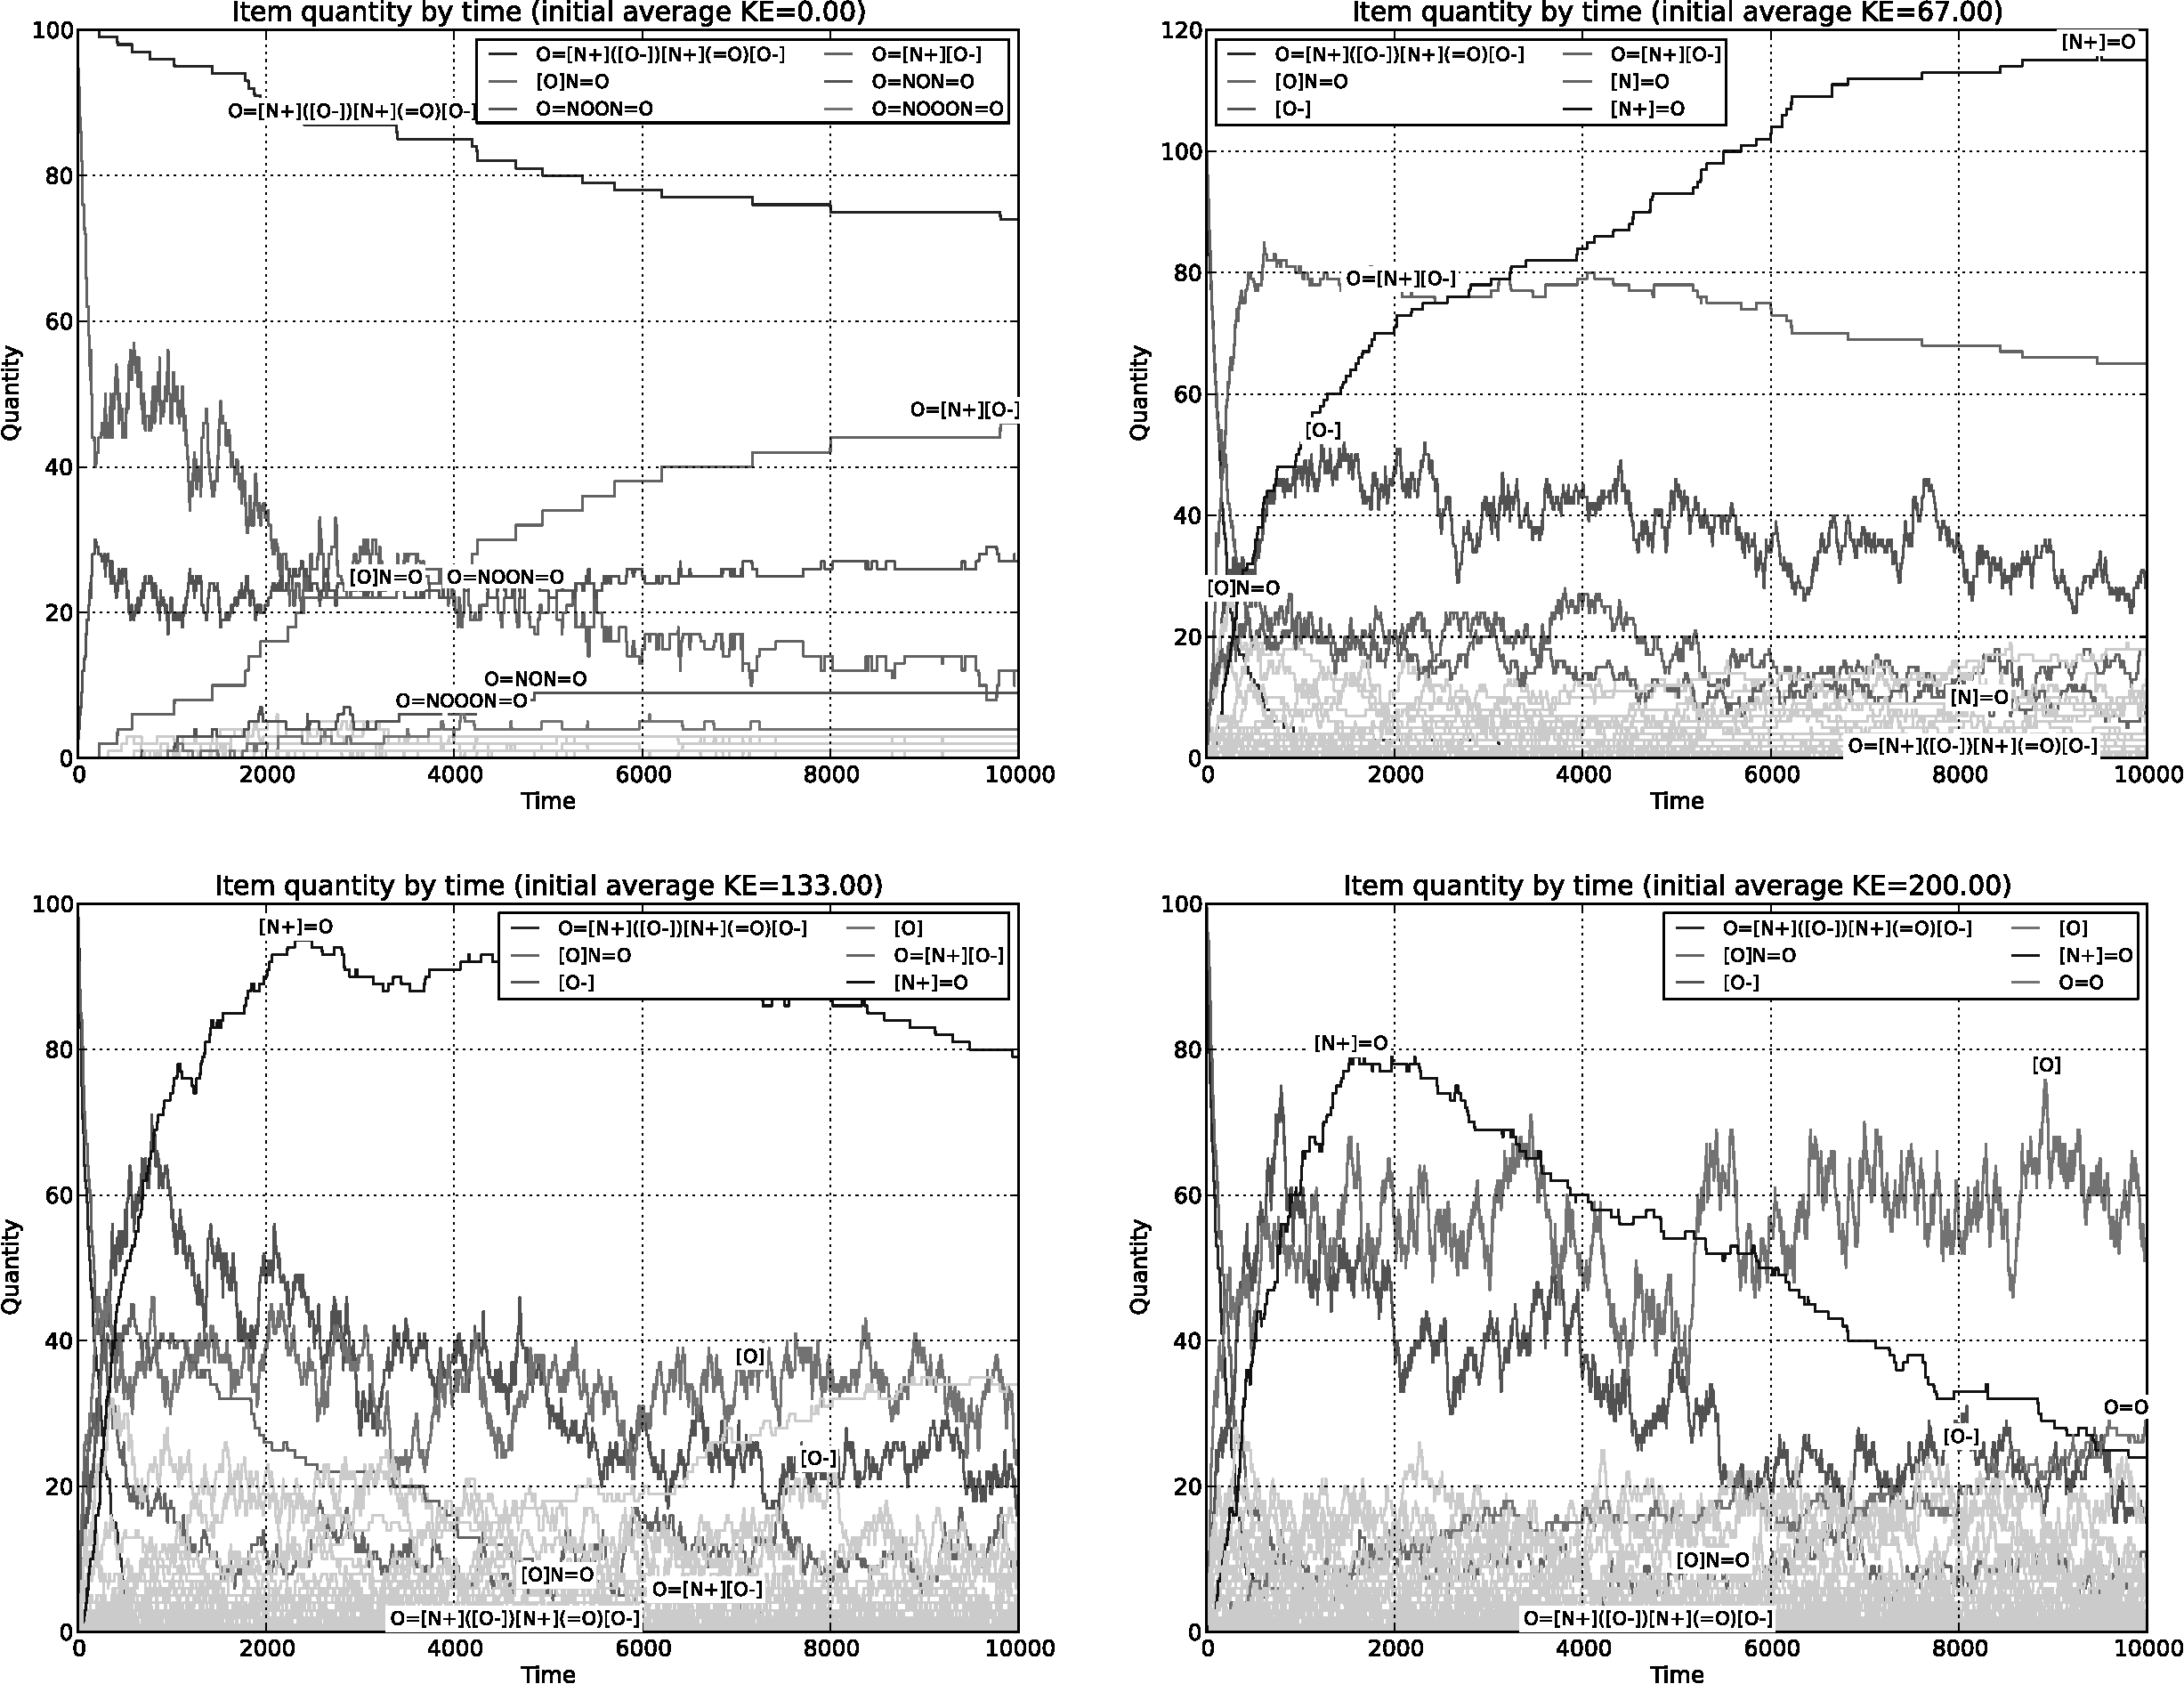
\includegraphics[width=\linewidth]{figures/results-test-N2O4a}
		\label{fig1}
	\end{center}
\end{figure}

\section{Results and Discussion}\label{results-and-discussion}

Beyond the initial transition period, both reactant sets showed results
essentially consistent with equilibrium. Population variability was high
in both cases, but more so for the N\textsubscript{2}O\textsubscript{4}
and 2NO\textsubscript{2} reactant set. In that case, some molecules
never reached a relatively constant population level (gradient of a
best-fit population line remained significantly non-zero.) The
fluctuations in the quantities of the other molecules are expected
according to our criteria, and result from the inherent variability in
reaction selection which causes the quantities to oscillate around a
norm.

With both reactant sets the model produced a significant number of
molecules which would be considered unstable in real-world chemistry
(such as O\textsuperscript{-} and O.) This is likely an artifact of the method
we use to generate reaction options, where a bond-break plus
bond-formation reaction -- moving through an intermediate unstable
ion -- occurs in our model as two separate reactions. As all molecules
currently react with equal likelihood, significant time can elapse
before the intermediate product reacts to form a stable product.

Both reactant sets showed clear differences in population composition
between the four initial kinetic energy levels. In the
H\textsubscript{2}, O\textsubscript{2} and H\textsubscript{2}O reactant set, no reactions
occurred at the zero energy level. This is expected from our energy
model as only bond-formations are possible without free kinetic energy.
With reactants of H\textsubscript{2}, O\textsubscript{2} and H\textsubscript{2}O no bond formations are possible,
confirmed by examining the bond options returned by the model for the
six possible combinations of initial reactants. By contrast, the
reactant set N\textsubscript{2}O\textsubscript{4} and
2NO\textsubscript{2} at energy zero contains one possible bond formation
reaction (in SMILES, [O]N=O.[O]N=O to O=N[O][O]N=O)
which can proceed without free kinetic energy. This then releases a
product which can also react, and so on, thus explaining the different
results between the reaction sets.

\section{Conclusions}\label{conclusions}

Our base artificial chemistry appears to be at least compatible with the
requirements for the future exploration of open-ended evolution. The
model is simpler than comparable alternatives, and the energy and
reaction models produce results consistent with our predictions for the
system's behaviour (with the exception of achieving equilibrium with the
N\textsubscript{2}O\textsubscript{4} and 2NO\textsubscript{2} reactant
set). An aspatial approach does however come with restrictions. Most
obviously, as there is no concept of proximity in the chemistry, there
can be no boundaries or membranes or even basic distinctions between
\emph{inside} and \emph{outside}. This is critical in biology but it is
unclear if this is equally important in non-biological systems. We
expect that experimental comparison between the aspatial and spatial
approaches in the course of our exploratory experiments will help to
clarify this.

\chapter{Reactant and Product Strategies}\label{reactant-and-product-strategies}

\section{Introduction}\label{introduction-5}

In this section we explore the following research questions:

\vspace{0.3cm}
\begin{minipage}[l]{0.95\textwidth}
	\begin{enumerate}[label=RQ\arabic*:]
		\item Is there a quantitative difference between different reactant and product selection strategies?
		\item Is there a combination of reactant and product selection strategies that leads to increased emergence as measured by cycles?
		\item Is emergence significantly affected by the values of other parameters of an Artificial Chemistry, such as initial kinetic energy or bond energies?
	\end{enumerate}
\end{minipage}
\vspace{0.3cm}

To the best of our knowledge, this is the first time that reaction and product selection strategies
in Artificial Chemistries have been experimentally compared.
Instead, the general approach of previous work, where there has been a quantitative evaluation,
has been to propose a particular strategy, build, and evaluate against the initial goals,
rather than against alternatives.

Our two primary factors, or independent variables, are $S_\mathrm{Reactant}$ and $S_\mathrm{Product}$.
We also introduce two secondary factors, overall reaction vessel energy ($E_\mathrm{Vessel}$) and
bond energy ($E_\mathrm{Bonds}$), to assess the sensitivity of the simulation to other parameters.
For simplicity of analysis, all of our factors are two-level, meaning they take one of two
possible levels, or values, in each run. The parameter values chosen for each level of
$E_\mathrm{Vessel}$ and $E_\mathrm{Bonds}$ were chosen as representative from a set of alternatives
used in initial exploratory experiments; in each case they allowed the simulation to run for an
extended period without running out of possible reactions (from lack of energy for example.)

\begin{table}
	\scriptsize
	\caption{Factors, or independent variables}\label{tbl:factors}
	\begin{tabular}{p{1.4cm}p{2.2cm}p{4.4cm}p{5.5cm}}
		\hline\noalign{\smallskip}
		Factor                & +1 value                          & -1 value                                                                                        & Description                                                    \\
		\hline
		\noalign{\smallskip}
		$S_\mathrm{Reactant}$ & Kinetic                           & Uniform                                                                                         & See Section \cref{reactant-selection-strategies}               \\
		$S_\mathrm{Product}$  & LeastEnergy                       & Uniform                                                                                         & See Section \cref{product-selection-strategies}                \\
		$E_\mathrm{Vessel}$   & 300                               & 100                                                                                             & Initial kinetic energy of each molecule in the reaction vessel \\
		$E_\mathrm{Bonds}$    & Single=50, Double=100, Triple=200 & Simplified real-world chemistry. Average values for Single=77.7, Double=148.2, and Triple=224.3 & Energy required to break a bond of the given type              \\
		\hline
	\end{tabular}
\end{table}

We concentrate on three related response, or dependent, variables -- Number of cycles, Length of longest cycle, and Count of most common cycle. All three are derived from a reconstruction of the network of reactions that occur during each experiment run, where every edge represents a specific reaction connecting a particular set of reactants with a particular set of products. Note that the nodes in the constructed network capture specific molecules, rather than molecular types or species that share the same chemical formula (as would be more usual in the construction of a Reaction Network for real-world chemistry.)

We exclude all unique cycles, and all cycles with three or fewer elements (for example, where a molecule loses, then regains, an atom repeatedly). Unique cycles by nature are unlikely to be representative; very short cycles on the other hand are so common as to dominate other more interesting cycles in any analysis.

\section{Experiment Design}
The experiments follow a full factorial design over four factors ($S_\mathrm{Reactant}$, $S_\mathrm{Product}$, $E_\mathrm{Vessel}$ and $E_\mathrm{Bonds}$), each at two levels, run in a randomized order, with three (3) replicates of each combination of factors executed in sequence before beginning the next combination. The first replicate of each combination starts with a predefined random seed incremented by one for each successive replicate of the same combination. The factor levels used are given in Table \cref{tbl:factors}.

Each replicate used the same initial population of 800 molecules, made up of 100 molecules each of [H][H], O=O, [O-][N+](=O)[N+]([O-])=O, and N(=O)[O] and 200 molecules each of O and O=C=O (all represented in SMILES \parencite{smiles}.) This initial population is somewhat arbitrary, although reasonable; given that ToyWorld is a strongly constructive chemistry, we would expect that any differences between initial populations would reduce as the simulation proceeds.

For details of the Artificial Chemistry, see \parencite{Young2013}. The chemistry makes use of some low-level components from RDKit \parencite{rdkit}, open-source software for cheminformatics. RDKit provides a number of useful capabilities, including format conversions to and from SMILES and graphical forms of molecules; standard sanity checks for molecular structure, and molecular manipulations. In ToyWorld, atoms are closely based on real-world chemistry atoms, and in fact are implemented as wrappers around the Atom definitions provided by RDKit; we allow any atom type provided by RDKit. Bonds in ToyWorld are represented by RDKit bonds, but the addition or subtraction mechanism makes use of the parameterised ToyWorld energy model.

\section{Results}
All replicates completed a set of 20,000 reactions; given the initial population size of 800 molecules, and from the summary of results below, we believe that this captures a representative set of reactions. This also simplifies the analysis as we can assume a balanced set of treatments in the statistical sense (that is, the sample sizes for all treatments are equal).

\begin{table}[htbp]
	\scriptsize
	\caption{Summary of results}\label{tbl:results}
	\begin{center}
		\begin{tabular}{lrrr}
			\hline\noalign{\smallskip}
			Statistic    & Number of cycles & Length of longest.cycle & Count of most common cycle \\
			\hline\noalign{\smallskip}
			\multicolumn{4}{c}{Reactions 4750 to 5000}\\
			\hline\noalign{\smallskip}
			Min.         & 0.00             & 0.00                    & 0.00                       \\
			1st Quartile & 0.00             & 0.00                    & 0.00                       \\
			Median       & 1.50             & 3.50                    & 2.50                       \\
			Mean         & 219.06           & 5.04                    & 215.80                     \\
			3rd Quartile & 91.25            & 7.75                    & 96.00                      \\
			Max.         & 5704.00          & 20.00                   & 2728.00                    \\
			\hline\noalign{\smallskip}
			\multicolumn{4}{c}{Reactions 9750 to 10000}\\
			\hline\noalign{\smallskip}
			Min.         & 0.00             & 0.00                    & 0.00                       \\
			1st Quartile & 0.00             & 0.00                    & 0.00                       \\
			Median       & 6.00             & 4.00                    & 6.00                       \\
			Mean         & 62.10            & 4.65                    & 169.21                     \\
			3rd Quartile & 68.75            & 8.25                    & 27.75                      \\
			Max.         & 526.00           & 13.00                   & 6684.00                    \\
			\hline\noalign{\smallskip}
			\multicolumn{4}{c}{Reactions 14750 to 15000}\\
			\hline\noalign{\smallskip}
			Min.         & 0.00             & 0.00                    & 0.00                       \\
			1st Quartile & 1.00             & 3.00                    & 2.00                       \\
			Median       & 5.00             & 4.50                    & 5.00                       \\
			Mean         & 27.17            & 4.79                    & 42.27                      \\
			3rd Quartile & 34.50            & 7.00                    & 16.25                      \\
			Max.         & 237.00           & 12.00                   & 862.00                     \\
			\hline\noalign{\smallskip}
			\multicolumn{4}{c}{Reactions 19750 to 20000}\\
			\hline\noalign{\smallskip}
			Min.         & 0.00             & 0.00                    & 0.00                       \\
			1st Quartile & 0.00             & 0.00                    & 0.00                       \\
			Median       & 3.50             & 4.00                    & 4.00                       \\
			Mean         & 20.04            & 3.90                    & 14.62                      \\
			3rd Quartile & 20.25            & 6.00                    & 13.25                      \\
			Max.         & 199.00           & 12.00                   & 216.00                     \\
			\hline
		\end{tabular}
	\end{center}
\end{table}%

A view of the results is given in Table \cref{tbl:results}: reaction networks built from the full dataset of 20,000 reactions can be too large for easy analysis. Instead, we choose to partition the reaction data into four equally spaced blocks of 250 reactions each and analyse each block independently.

\TODO{convert to ggplot2}

\TODO{convert to ggplot2}
<<cyclesbypartition, pdfcrop=TRUE, echo=FALSE, cache=TRUE, fig.show='hold', fig.cap='Cycles by reaction partition (starting reaction number for each partition along x-axis)'>>=
df<-load.toyworld("results/EvaluatorActualCycles.out")
par(mfrow=c(1,3),cex=0.5)
plot(df$Number.of.cycles~df$Partition.Start, main="Cycle numbers by Partition", ylab="Number of cycles")
plot(df$Length.of.longest.cycle~df$Partition.Start, main="Cycle length by Partition", ylab="Length of longest cycle")
plot(df$Count.of.most.common.cycle~df$Partition.Start, main="Cycle count by Partition", ylab="Count of most common cycle")
@
\label{fig:partitions}

%\begin{figure}[h]
%\centering
%	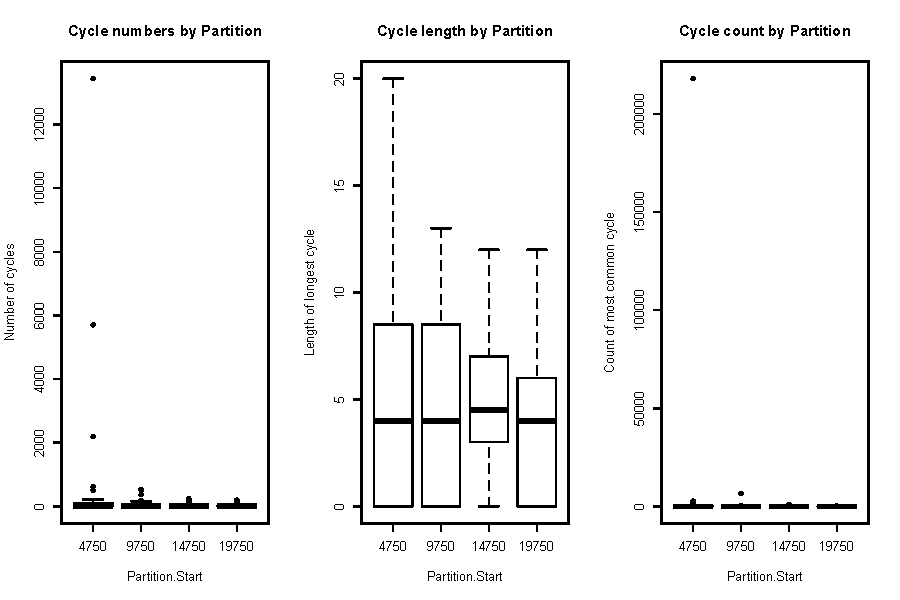
\includegraphics[width=0.95\linewidth]{figures/partitions}
%	\caption{Cycles by reaction partition (starting reaction number for each partition along x-axis)}
%	\label{fig:partitions}
%\end{figure}

% No R code...
\begin{figure}[h]
	\centering
	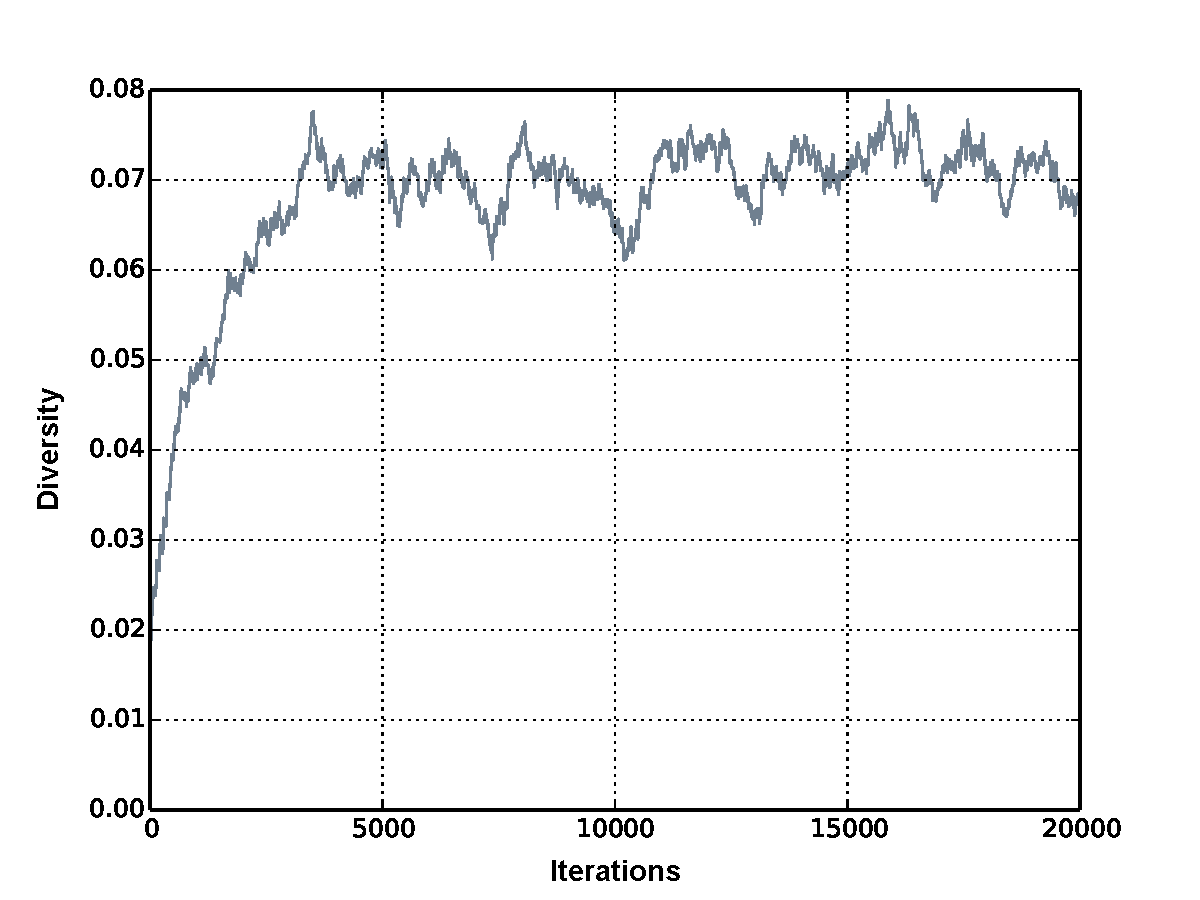
\includegraphics[width=0.45\linewidth]{figures/PlotMolecularDiversity-strategies-12-0}
	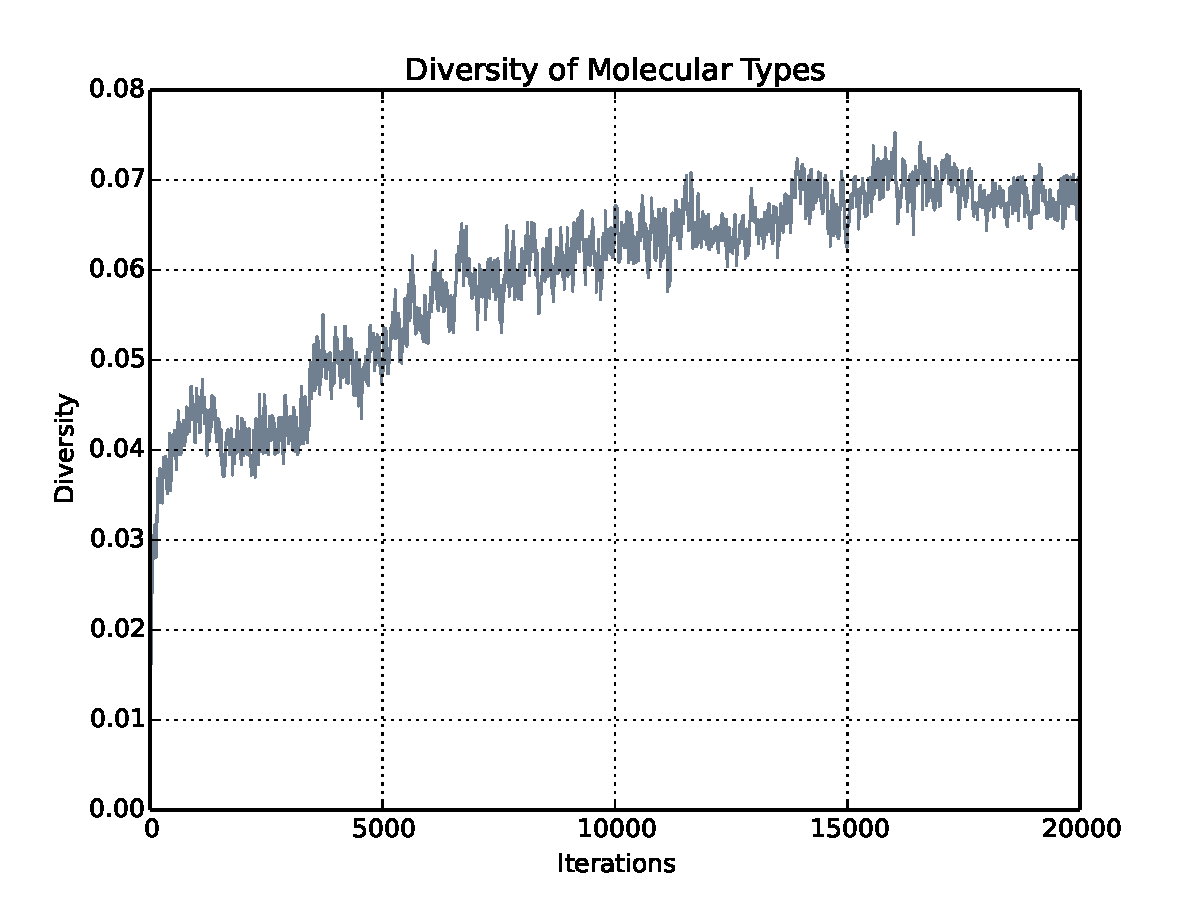
\includegraphics[width=0.45\linewidth]{figures/PlotMolecularDiversity-strategies-16-1}
	\caption{Diversity for Replicates 12-0 and 16-1}\label{fig:diversity}
\end{figure}

\subsection{Analysis and Discussion}
Figure \cref{fig:cyclesbypartition} suggests that the first partition, representing the vessel a quarter of the way into its lifespan, is quantitatively different from the other three partitions, with a significantly greater range for all three response variables. Intuitively this corresponds with an initial period where the diversity in the reaction vessel rapidly increases from the limited starting set of molecules, as seen in some (e.g, Figure \cref{fig:diversity}) but not necessarily all of the replicates. Diversity here is measured by (average molecular quantity)$^{-1}$. All following sections therefore exclude data from the first partition of reaction numbers from 4750 to 5000.

\TODO{convert to ggplot2}
<<reactantstrategy, pdfcrop=TRUE, echo=FALSE, cache=TRUE, fig.show='hold', fig.cap='Response by Reactant Strategy '>>=
df <- subset(df,df$Partition.Start != "4750")
par(mfrow=c(1,3),cex=0.5)
boxplot(Number.of.cycles~Product.Strategy, data=df, main="Cycle numbers by Product Strategy", names=c("Uniform","Energy"), ylab="Number of cycles")
boxplot(Length.of.longest.cycle~Product.Strategy, data=df, main="Cycle length by Product Strategy", names=c("Uniform","Energy"), ylab="Length of longest cycle")
boxplot(Count.of.most.common.cycle~Product.Strategy, data=df, main="Cycle count by Product Strategy",names=c("Uniform","Energy"), ylab="Count of most common cycle")
@

%\begin{figure}[t]
%\centering
%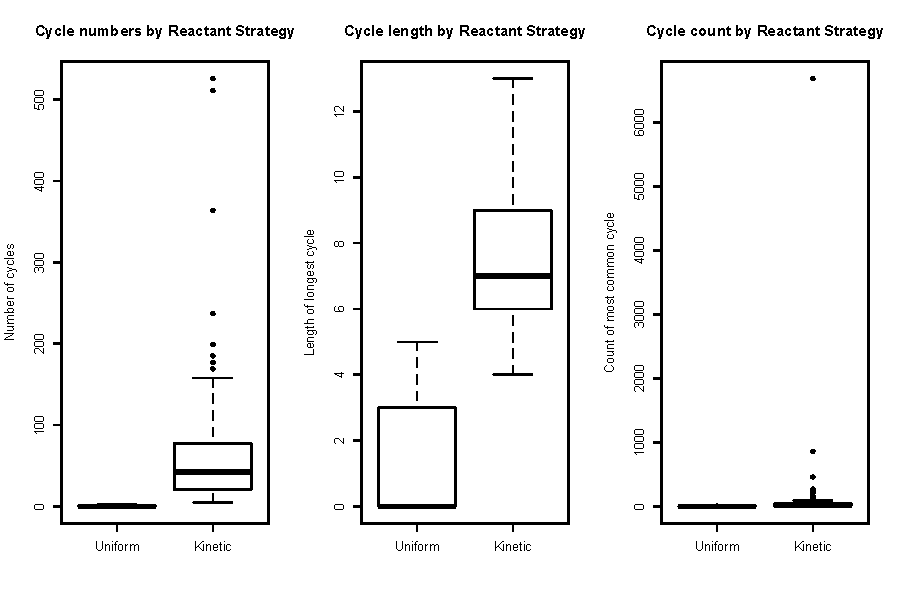
\includegraphics[width=0.95\linewidth]{figures/reactant_strategy}
%\caption{Response by $S_\mathrm{Reactant}$}
%\label{fig:reactant_strategy}
%\end{figure}

\TODO{convert to ggplot2}
<<productstrategy, pdfcrop=TRUE, echo=FALSE, cache=TRUE, fig.show='hold', fig.cap='Response by Product Strategy '>>=
par(mfrow=c(1,3),cex=0.5)
boxplot(Number.of.cycles~Reactant.Strategy, data=df, main="Cycle numbers by Reactant Strategy", names=c("Uniform","Kinetic"), ylab="Number of cycles")
boxplot(Length.of.longest.cycle~Reactant.Strategy, data=df, main="Cycle length by Reactant Strategy", names=c("Uniform","Kinetic"), ylab="Length of longest cycle")
boxplot(Count.of.most.common.cycle~Reactant.Strategy, data=df, main="Cycle count by Reactant Strategy",names=c("Uniform","Kinetic"), ylab="Count of most common cycle")
@

%\begin{figure}[t]
%\centering
%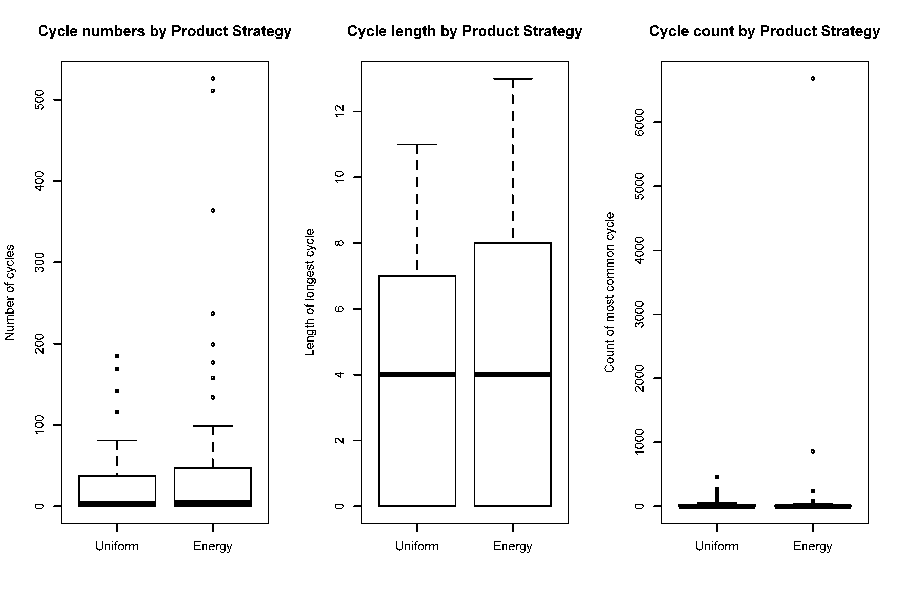
\includegraphics[width=0.95\linewidth]{figures/product_strategy}
%\caption{Response by $S_\mathrm{Product}$}
%\label{fig:product_strategy}
%\end{figure}

\subsection{RQ1: Is there a quantitative difference between the different reactant and product selection strategies?}
From visual inspection of Figure \cref{fig:reactantstrategy}, there appears to be a significant difference between the Uniform and Kinetic reactant selection strategies for number and length of cycles. Kinetic reactant selection seems to result in significantly higher levels of emergent behaviour than Uniform reactant selection. Similarly, from Figure \cref{fig:productstrategy}, there is very little apparent difference between the two product strategies, Uniform selection and Least Energy selection.

We use ANOVA (Analysis of Variance) to further examine the relationship of $S_\mathrm{Reactant}$ and $S_\mathrm{Product}$ to the response variables using a two-factor with two-levels (2x2) model (degrees of freedom=1) with interaction effects. There is a highly significant difference (p\textless 0.001) between the Uniform and Kinetic reactant selection strategies when comparing the number of cycles (f-value=40.442) and length of cycles (f-value=361.891) (confirming the impression given by Figure \cref{fig:reactantstrategy}), although again without difference for the count of the most common cycle. The effect of $S_\mathrm{Product}$ on cycle number and length is also significant (f-value=4.050 and 5.705 respectively, p\textless 0.05) and there is a first-order interaction between $S_\mathrm{Reactant}$ and $S_\mathrm{Product}$ for number of cycles (f-value=4.011, p\textless 0.05).

\TODO{convert to ggplot2}
<<reactantproductcombination, pdfcrop=TRUE, echo=FALSE, cache=TRUE, out.width='0.30\\linewidth', fig.height=4, fig.show='hold', fig.cap='Effect of the combination of Reactant and Product Strategies on Response Variables '>>=
boxplot(Number.of.cycles ~ Reactant.Strategy+Product.Strategy, data=df,  log="y", ylim=c(1,6000),names=c("Uniform:Uniform","Kinetic:Uniform","Uniform:Energy","Kinetic:Energy"))
boxplot(Length.of.longest.cycle ~ Reactant.Strategy+Product.Strategy, data=df,  log="y", ylim=c(1,6000),names=c("Uniform:Uniform","Kinetic:Uniform","Uniform:Energy","Kinetic:Energy"))
boxplot(Count.of.most.common.cycle ~ Reactant.Strategy+Product.Strategy, data=df, log="y", ylim=c(1,6000), names=c("Uniform:Uniform","Kinetic:Uniform","Uniform:Energy","Kinetic:Energy"))
@

%\begin{figure}[t]
%\centering
%\subcaptionbox{Cycle Count by Strategy Combination %($S_\mathrm{Reactant}$:$S_\mathrm{Product}$)\label{fig:cycle_count}}[0.45\linewidth][r]{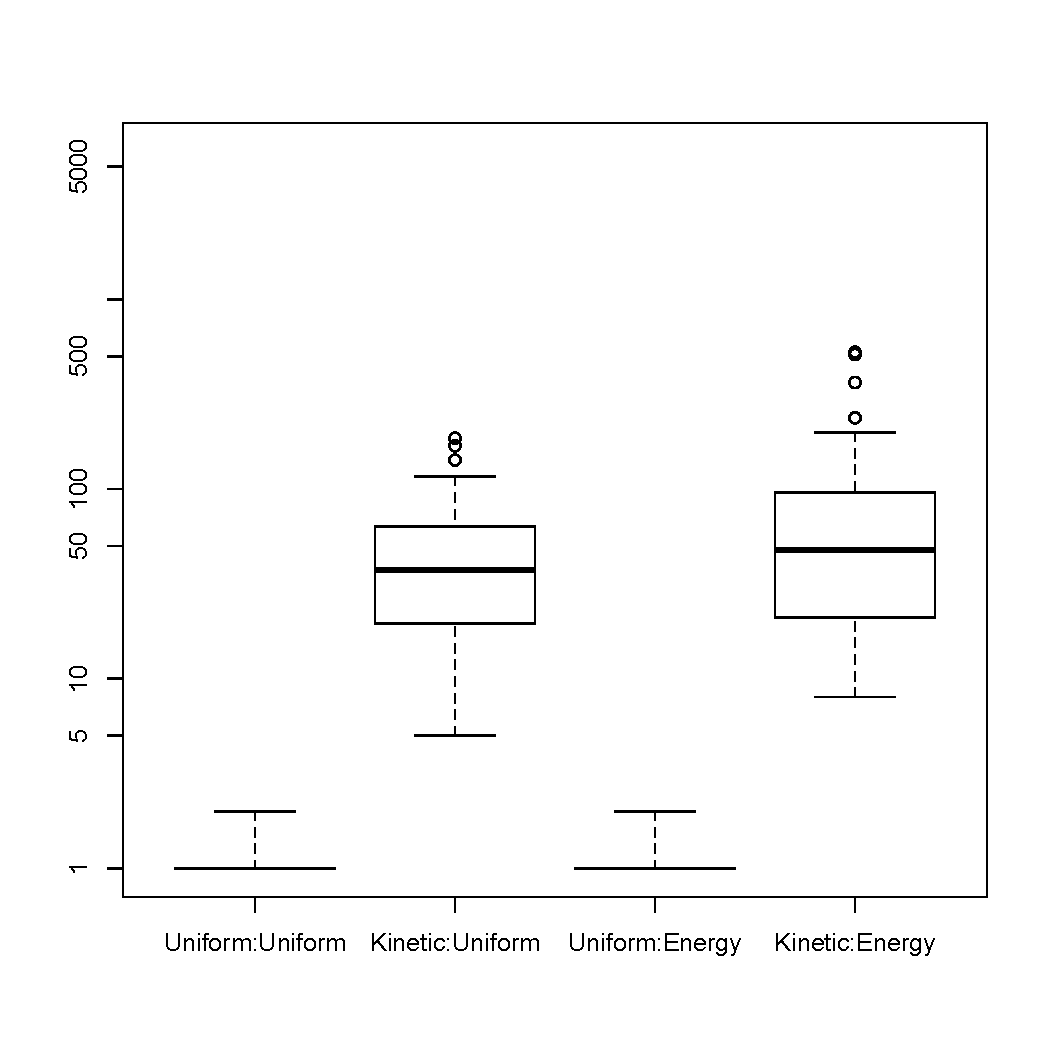
\includegraphics[width=0.45\linewidth]{figures/cycle_count}}
%\subcaptionbox{Cycle Length by Strategy Combination %($S_\mathrm{Reactant}$:$S_\mathrm{Product}$)\label{fig:cycle_length}}[0.45\linewidth][l]{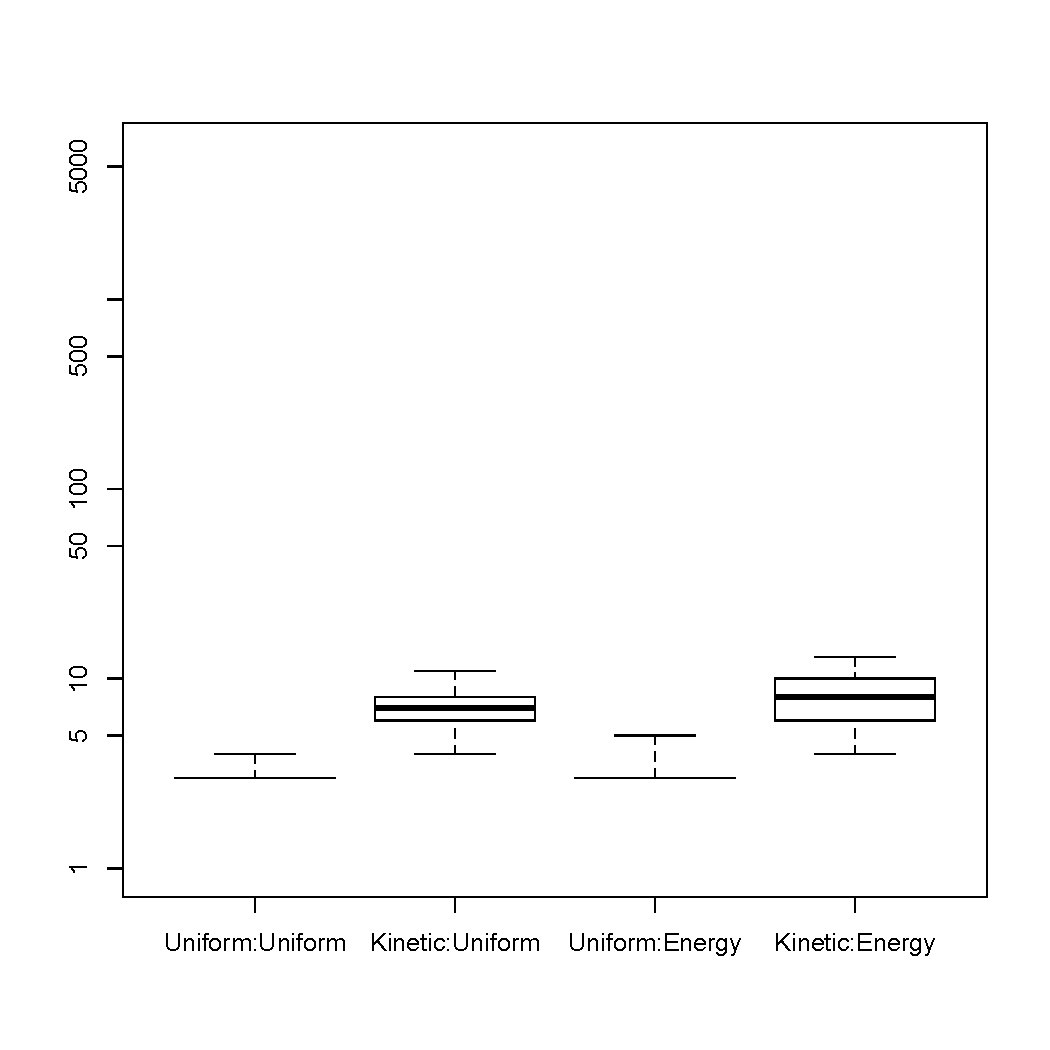
\includegraphics[width=0.45\linewidth]{figures/cycle_length}}
%\subcaptionbox{Count of Most Common Cycle by Strategy Combination %($S_\mathrm{Reactant}$:$S_\mathrm{Product}$)\label{fig:cycle_common}}[0.45\linewidth][r]{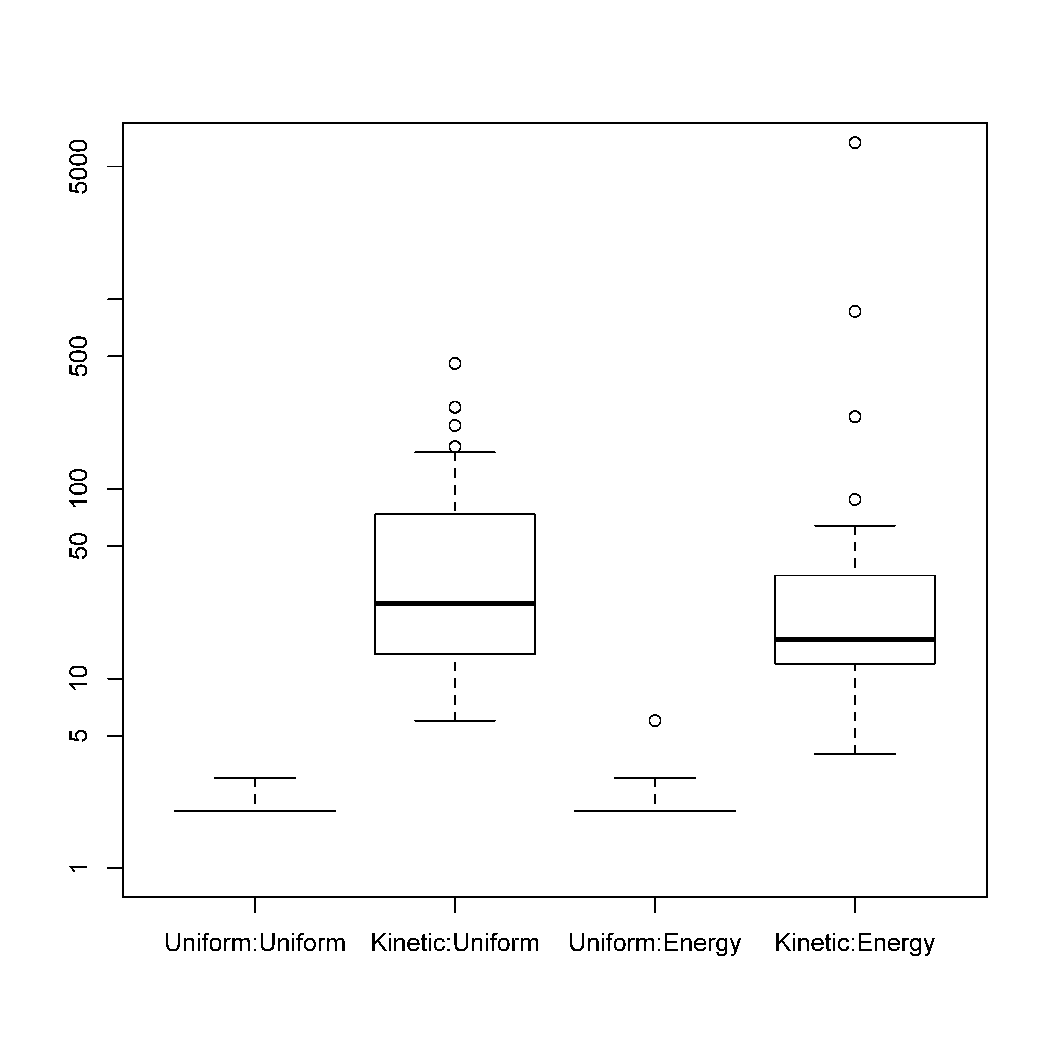
\includegraphics[width=0.45\linewidth]{figures/cycle_common}}
%\caption{Effect of the combination of $S_\mathrm{Reactant}$ and $S_\mathrm{Product}$ on Response Variables}
%\end{figure}

\subsection{RQ2: Is there a combination of reactant and product selection strategies that leads to increased emergence as measured by cycles?}

From Figure \cref{fig:reactantproductcombination} it is clear that there is no significant relationship between strategy and the number of occurrence of the most common cycle. However, it seems that such a relationship does exist for the number and length of cycles, with the strongest effect as a result of $S_\mathrm{Reactant}$, and a lesser effect from the choice of $S_\mathrm{Product}$.

We conclude that the greatest levels of emergence are likely to be seen with the combination of $S_\mathrm{Reactant} = \mathrm{Kinetic}$ and $S_\mathrm{Product} = \mathrm{LeastEnergy}$.

\subsection{RQ3: Is emergence significantly affected by the values of other parameters of an Artificial Chemistry, such as initial kinetic energy or bond energies?}

We constructed a two-factor with two-levels (2x2) ANOVA model (degrees of freedom=1) with interaction effects to examine the relationship of the independent variables $E_\mathrm{Vessel}$ and $E_\mathrm{Bonds}$ to the response variables, and applied it to our dataset (summarised in Table \cref{tbl:results}). $E_\mathrm{Bonds}$ is significant (f-value=4.221, p\textless 0.05) to number of cycles. No other significant relationships exist.

\section{Conclusions}
The choice of $S_\mathrm{Reactant}$ is critical to the behaviour of an emergent Artificial Chemistry; $S_\mathrm{Product}$ on the other hand appears to have a lesser effect on the emergence of cycles in our experiments. Furthermore, $S_\mathrm{Reactant} = \mathrm{Kinetic}$ is more effective for cycle emergence than $S_\mathrm{Reactant} = \mathrm{Uniform}$.

The most significant limitation of our analysis overall is that the values chosen for the high and low values of $E_\mathrm{Bonds}$ make it impossible to determine the cause of the difference observed in RQ3. There are two alternative explanations: first, the energy required to make or break bonds is simply different between the two factor levels; second, in the low factor level, based on real-world values, the bond make and break energies for even a single bond vary depending on the atoms involved, while in the high factor level these values are consistent for all bonds of the same degree. To distinguish between the two explanations we would need at least the average levels at each degree to be the same for each factor; this is a suggestion for a future experiment.

\chapter{Discussion}

\TODO{Autocatalysis as a very simple form of inheritance and reproduction without variation. Pathway perhaps from this towards a form with variation, when hypothesis-2 kicks in...}

\part{Conclusions}\label{the-search-for-creativity}

\chapter{TODO-Introduction}

The parameters themselves become endogenized, in the case of \emph{Fitness} into an implicit relative fitness and for \emph{Fidelity} into the outcome of the copying/variation mechanism.

``Fitness determines context''--in contrast to Part 2, the entity affects its environment

Fitness is relative to a context or niche. Creativity is where the
entity changes niche or context--either by moving to a new niche, or
creating or modifying one

Creativity requires a feedback loop between entity and environment--a
common representation for both so that they can interact (and entities
can interact with other entities, and elements within the enviroment
with other elements\ldots{})

Other open areas--workings of selection

Hints--e.g., Taylor, Van Valen\ldots{}--regarding resource
competition, when individuals are embedded (required for single set of
omnipotent rules)

Hypothesis--Resource competition as the mechanism of selection

\begin{itemize}
	\item
 Does this simplify/remove choices? (as we earlier saw with
 reproduction/replication?)
	\item
 Addition/Removal follows automatically
\end{itemize}

\section{Requirements for chemistry}\label{requirements-for-chemistry}

\section{Previous work}\label{previous-work-1}

\section{Match to requirements}\label{match-to-requirements}

\section{Chemistry selection}\label{chemistry-selection}

\quote{
	Standish (2003), which is that openendedness depends fundamentally on
the continual production of novelty.}
{\autocite{Soros2014}}

\section{\texorpdfstring{What is interesting? Require formal defn for ``proof''\ldots{}}{What is interesting? Require formal defn for proof\ldots{}}}\label{what-is-interesting-require-formal-defn-for-proof}

Levels are interesting in biology (should defn encompass biology or
focus on CS?)

Interesting seems to be different search space, not just bigger space.
What about better search of same space? Is that interesting?

\quote{\ldots{}the processes associated with the major transitions are an
	automatic consequence of mutation and selection, due to the generation
of higher levels of selection due to spatial self-organization.}
{\autocite{Hogeweg1998}}

\begin{itemize}
	\item
 although somewhat quantified by scope (spatial structures e.g.,
 waves/spirals) and lack of fourth of element of Maynard-Smith:1995lw -
 ``transition from limited inheritance to universal inheritance''
\end{itemize}

Evolutionary mechanism from earlier is made up of variation and
selection elements

Evolutionary mechanism must be itself capable of improvement

\begin{itemize}
	\item
 Levels of selection requires changes in mechanism
	\item
 And levels are correlated with surprise--major transitions in
 evolution (Maynard-Smith:1995lw) (although specifics here are
 biologically derived)
	\item
 e.g., Mechanism of evolution must be itself evolvable; individuals and
 environment interact to give new ways of producing new individuals.
 Dynamics required for novelty-generation (Nellis2014)
	\item
 Evolvable mechanism; implies embodied, or endogenous--mechanism must
 be capable of evolvable under same conditions as shown earlier for
 evolutionary potential
	\item
 Inheritable variation under selection
 
 \begin{itemize}
	      	\item
 	      If intrinsic selection, then mechanism for
 	      inheritance/variation/selection should be expressed in same language
 	      as other evolvable elements--a common rule set or chemistry. If
 	      different, then cannot have interactions between other elements and
 	      evolutionary mechanism--limited EvoEvo
 \end{itemize}
\end{itemize}

Show that given 1) OEE evolutionary system from above 2) capable of
self-modification--process evolution, capable of ``interesting''

Sufficient condition

\textit{Hypothesis 4}: Endogenous selection and variation under evolutionary control sufficient for ``novelty-generation'' in evolution

From earlier Hypothesis 3, V+S-\textgreater{}E

Endogenous selection by resource competition

World = Elements + Interactions

More complex interactions emerge (constructive)

\begin{itemize}
	\item
 Some compositions actively evolve (strong selection), all others
 potentially affected (weak selection and no selection)
	\item
 How do compositions form and how are they maintained? Some rule in
 world must impose a form of bias or asymmetry to allow differences to
 develop. In biology, locality of effect is one example
	\item
 Compositions rely on external-to-them elements and lacking those,
 cannot maintain themselves. Growth and maintenance results from
 success in resource competition
\end{itemize}

Variation under evolutionary control

\begin{itemize}
	\item
 A' = f(A), if f() fixed then must be capable of generating all future
 variation. Alternative is a f() which is not-fixed, but is itself
 capable of variation. What type of variation?
	\item
 Needs to be novel and open-ended itself!
	\item
 EvoEvo simplest--same mechanism
	\item
 Shared mechanism for I and V--capable of introducing some V during I
	\item
 V must be exposed to S
	\item
 Feedback loop--V refined by S
	\item
 Prediction: V changes over time. In more detailed models, form of V
 may change over time (not possible without an EvoEvo mechanism)
	\item
 Prediction: correlation between parent and offspring properties is highest
 in unchanging (stable) environments, and lowest in varying ones. In
 systems without variation under evolutionary control, correlation is
 unchanging. (in previous section, correlation modelled as under
 evolutionary control with degree of correlation as endogenous
 parameter)
\end{itemize}

\subsection{Tests for evolutionary activity}\label{tests-for-evolutionary-activity-1}

Sustainability may be undecidable--Wiedermann:2005ys

Alife community--Channon, etc

Population measures e.g., Vasas2015

Artificial selection

Moran's test

Search mechanism--thermodynamic or ergodic search vs evolutionary
search (implied by Rasmussen2004)

Local entropy (implied by Adami2015)

Measure of OEE -
http://link.springer.com/article/10.1007\%2Fs11084-012-9309-y

\chapter{TODO-Discussion and Conclusions}\label{discussion-and-conclusions}

We have shown that:
\begin{itemize}
	\item Selection and Variation are sufficient for Evolution in an Artificial System
	\item Such a system is capable of adjusting to changing environments without preselection of parameters
	\item Such a system can be implemented in an Artificial Chemistry
\end{itemize}

And therefore that open-ended evolution is possible in an Artificial Chemistry.

\TODO{ link OEE to selection and variation from work in \cref{the-search-for-creativity}}

Requires a series of steps--akin to OOL where single-step
astronomically unlikely (single RNA strand probability about 10E-60,
based on 100 monomers--\autocite{Pascal2013})

\section{Step 1--demonstration of Autocatalytic activity}\label{step-1 -- demonstration-of-autocatalytic-activity}

Previous work

\begin{itemize}
	\item
 \autocite{Gordon-Smith2013}--Quite complex systems for replication demonstrated
 in SimSoup-2, handcrafted molecules
	\item
 \autocite{Bagley1990}
	\item
 GARD--\autocite{Segre1998}
	\item
 \autocite{Ono2002}--Boid-like rules in Lattice Artificial Chemistry leads to
 membrane formation. Fixed types of particles with associated
 hydrophobic/hydrophilic/neutral class (with orientation). Fixed
 reaction paths to form an autocatalytic set of reactions
	\item
 \autocite{Huning2000}
\end{itemize}

\section{Step 2--demonstration of selection between ACS}\label{step-2 -- demonstration-of-selection-between-acs}

Test of evolution under selection versus drift- artificial selection -
show response to selective pressure

\section{Step 3--Evolution in an artificial chemistry}\label{step-3 -- evolution-in-an-artificial-chemistry}

\section{Alternative explanations}\label{alternative-explanations}

\begin{itemize}
	\item
 Thermodynamics
	\item
 Experimental/Model bias (e.g., discovered bias of GARD inheritance
 model)
\end{itemize}

\section{Tests for evolutionary activity}\label{tests-for-evolutionary-activity}

\begin{itemize}
	\item
 Sustainability may be undecidable--\autocite{Wiedermann:2005ys}
	\item
 Alife community--\autocite{Channon:2006st}, etc
	\item
 Population measures e.g., \autocite{Vasas2015}
	\item
 Artificial selection
	\item
 Moran's test
	\item
 Search mechanism--thermodynamic or ergodic search vs evolutionary
 search (implied by \autocite{Rasmussen2004})
	\item
 Local entropy (implied by \autocite{Adami2015})
	\item
 Measure of OEE--\autocite{Markovitch2012}
\end{itemize}

\section{Tests for sufficient conditions}\label{tests-for-sufficient-conditions}

\begin{itemize}
	\item
 Remove a condition (e.g., \autocite{Soros2014})
\end{itemize}
